\documentclass[presentation,xcolor={table},9pt]{beamer}

\usepackage{adjustbox}
\usepackage{algorithm}
\usepackage{algpseudocode}
\usepackage{amsfonts}
\usepackage{amsmath}
\usepackage{amssymb}
\usepackage{amsthm}
\usepackage{bookmark}
\usepackage{booktabs}
\usepackage[makeroom]{cancel}
\usepackage[american]{circuitikz}
\usepackage{cite}
% \usepackage{fixmath}
\usepackage[acronym]{glossaries-extra}
\usepackage{hyperref}
\usepackage{import}
\usepackage{mathtools}
\usepackage{microtype}
\usepackage[short]{optidef}
\usepackage{pgfplots}
\usepackage{ragged2e}
\usepackage{siunitx}
\usepackage{stfloats}
\usepackage[caption=false,font=footnotesize,subrefformat=parens,labelformat=parens]{subfig}
\usepackage{tabularx}
\usepackage{tikz}
\usepackage{graphicx}
\usepackage{epstopdf}
\usepackage{multirow}
\usepackage{booktabs}
\usepackage{lastpage}
\usepackage{caption}
\setbeamerfont{caption}{size=\footnotesize}
\captionsetup[figure]{labelformat=empty}
\usefonttheme[onlymath]{serif}

\makeatletter
\@addtoreset{subfigure}{framenumber}
\makeatother

\makeatletter
\newcommand{\forcealgorithm}{\let\@latex@error\@gobble}
\makeatother

% footnote
\newcommand\blfootnote[1]{%
\begingroup
\renewcommand\thefootnote{}\footnote{#1}%
\addtocounter{footnote}{-1}%
\endgroup
}

% amsthm
\newtheorem{proposition}{Proposition}
\newtheorem{remark}{Remark}
% \newtheorem{lemma}{Lemma}
% \newtheorem{corollary}{Corollary}[proposition]

% PGF/TikZ
\pgfplotsset{compat=1.18}
\usepgfplotslibrary{fillbetween,groupplots,patchplots}
\usetikzlibrary{arrows,arrows.meta,automata,backgrounds,calc,math,matrix,patterns,plotmarks,positioning,shapes,angles,quotes}
\usetikzlibrary{decorations.pathmorphing,decorations.pathreplacing,decorations.markings,decorations.shapes,shapes.geometric}

% glossaries-extra
\glsdisablehyper
\setabbreviationstyle[acronym]{long-short}
\newacronym{ai}{AI}{Artificial Intelligence}
\newacronym{af}{AF}{Amplify-and-Forward}
\newacronym{ambc}{AmBC}{Ambient Backscatter Communication}
\newacronym{am}{AM}{Arithmetic Mean}
\newacronym{ao}{AO}{Alternating Optimization}
\newacronym{ap}{AP}{Access Point}
\newacronym{apm}{APM}{Amplitude-Phase Modulation}
\newacronym{awgn}{AWGN}{Additive White Gaussian Noise}
\newacronym{bbc}{BBC}{Bistatic Backscatter Communication}
\newacronym{bcd}{BCD}{Block Coordinate Descent}
\newacronym{bc}{BackCom}{Backscatter Communication}
\newacronym{bd}{BD}{Beyond-Diagonal}
\newacronym{ber}{BER}{Bit Error Rate}
\newacronym{bibo}{BIBO}{Binary-Input Binary-Output}
\newacronym{bls}{BLS}{Backtracking Line Search}
\newacronym{bpcu}{\si{bpcu}}{bits per channel use}
\newacronym{bpsphz}{\si{bps/Hz}}{bits per second per Hertz}
\newacronym{clt}{CLT}{Central Limit Theorem}
\newacronym{cp}{CP}{Canonical Polyadic}
\newacronym{cr}{CR}{Cognitive Radio}
\newacronym{cscg}{CSCG}{Circularly Symmetric Complex Gaussian}
\newacronym{csit}{CSIT}{Channel State Information at the Transmitter}
\newacronym{csi}{CSI}{Channel State Information}
\newacronym{cw}{CW}{Continuous Waveform}
\newacronym{d2d}{D2D}{Device-to-Device}
\newacronym{dcmc}{DCMC}{Discrete-input Continuous-output Memoryless Channel}
\newacronym{dc}{DC}{Direct Current}
\newacronym{df}{DF}{Decode-and-Forward}
\newacronym{dmc}{DMC}{Discrete Memoryless Channel}
\newacronym{dmmac}{DMMAC}{Discrete Memoryless Multiple Access Channel}
\newacronym{dmtc}{DMTC}{Discrete Memoryless Thresholding Channel}
\newacronym{dof}{DoF}{Degree of Freedom}
\newacronym{dp}{DP}{Dynamic Programming}
\newacronym{eirp}{EIRP}{Effective Isotropic Radiated Power}
\newacronym{fdma}{FDMA}{Frequency-Division Multiple Access}
\newacronym{fpga}{FPGA}{Field-Programmable Gate Array}
\newacronym{gm}{GM}{Geomtric Mean}
\newacronym{gp}{GP}{Geometric Programming}
\newacronym{ic}{IC}{Interference Channel}
\newacronym{iid}{i.i.d.}{independent and identically distributed}
\newacronym{im}{IM}{Index Modulation}
\newacronym{ioe}{IoE}{Internet of Everything}
\newacronym{iot}{IoT}{Internet of Things}
\newacronym{kkt}{KKT}{Karush-Kuhn-Tucker}
\newacronym{los}{LoS}{Line-of-Sight}
\newacronym{m2m}{M2M}{Machine-to-Machine}
\newacronym{mac}{MAC}{Multiple Access Channel}
\newacronym{mbc}{MBC}{Monostatic Backscatter Communication}
\newacronym{mc}{MC}{Multiplication Coding}
\newacronym{mimo}{MIMO}{Multiple-Input Multiple-Output}
\newacronym{miso}{MISO}{Multiple-Input Single-Output}
\newacronym{ml}{ML}{Maximum-Likelihood}
\newacronym{mmse}{MMSE}{Minimum Mean-Square-Error}
\newacronym{mrc}{MRC}{Maximal Ratio Combining}
\newacronym{mrt}{MRT}{Maximum Ratio Transmission}
\newacronym{mse}{MSE}{Mean-Square Error}
\newacronym{nlos}{NLoS}{Non-Line-of-Sight}
\newacronym{noma}{NOMA}{Non-Orthogonal Multiple Access}
\newacronym{ofdm}{OFDM}{Orthogonal Frequency-Division Multiplexing}
\newacronym{pc}{PC}{Point-to-point Channel}
\newacronym{pdf}{PDF}{Probability Density Function}
\newacronym{pga}{PGA}{Projected Gradient Ascent}
\newacronym{pin}{PIN}{Positive Intrinsic Negative}
\newacronym{psk}{PSK}{Phase Shift Keying}
\newacronym{ps}{PS}{Power Splitting}
\newacronym{qam}{QAM}{Quadrature Amplitude Modulation}
\newacronym{qos}{QoS}{Quality of Service}
\newacronym{r-e}{R-E}{Rate-Energy}
\newacronym{rcg}{RCG}{Riemannian Conjugate Gradient}
\newacronym{rfid}{RFID}{Radio-Frequency Identification}
\newacronym{rf}{RF}{Radio-Frequency}
\newacronym{ris}{RIS}{Reconfigurable Intelligent Surface}
\newacronym{sca}{SCA}{Successive Convex Approximation}
\newacronym{sc}{SC}{Superposition Coding}
\newacronym{sdma}{SDMA}{Space-Division Multiple Access}
\newacronym{sdp}{SDP}{Semi-Definite Programming}
\newacronym{sdr}{SDR}{Semi-Definite Relaxation}
\newacronym{sic}{SIC}{Successive Interference Cancellation}
\newacronym{simo}{SIMO}{Single-Input Multiple-Output}
\newacronym{sinr}{SINR}{Signal-to-Interference-plus-Noise Ratio}
\newacronym{siso}{SISO}{Single-Input Single-Output}
\newacronym{smawk}{SMAWK}{Shor-Moran-Aggarwal-Wilber-Klawe}
\newacronym{star}{STAR}{Simultaneous Transmission and Reflection}
\newacronym{smf}{SMF}{Scaled Matched Filter}
\newacronym{snr}{SNR}{Signal-to-Noise Ratio}
\newacronym{sr}{SR}{Symbiotic Radio}
\newacronym{svd}{SVD}{Singular Value Decomposition}
\newacronym{swipt}{SWIPT}{Simultaneous Wireless Information and Power Transfer}
\newacronym{tdma}{TDMA}{Time-Division Multiple Access}
\newacronym{ts}{TS}{Time Switching}
\newacronym{ue}{UE}{User Equipment}
\newacronym{wf}{WF}{Water-Filling}
\newacronym{wit}{WIT}{Wireless Information Transfer}
\newacronym{wpcn}{WPCN}{Wireless Powered Communication Network}
\newacronym{wpt}{WPT}{Wireless Power Transfer}
\newacronym{wsn}{WSN}{Wireless Sensor Network}
\newacronym{wsr}{WSR}{Weighted Sum-Rate}
\newacronym{zf}{ZF}{Zero-Forcing}
\newacronym{lc}{LC}{Low-Complexity}
\newacronym{ble}{BLE}{Bluetooth Low Energy}
\newacronym{lora}{LoRa}{Long Range}
\newacronym{lorawan}{LoRaWAN}{Long Range Wide Area Network}
\newacronym{pae}{PAE}{Power-Added Efficiency}
\newacronym{papr}{PAPR}{Peak-to-Average Power Ratio}
\newacronym{fsk}{FSK}{Frequency-Shift Keying}
\newacronym{css}{CSS}{Chirp Spread Spectrum}
\newacronym{dsss}{DSSS}{Direct-Sequence Spread Spectrum}
\newacronym{fhss}{FHSS}{Frequency-Hopping Spread Spectrum}
\newacronym{rz}{RZ}{Return-to-Zero}
\newacronym{nrz}{NRZ}{Non-Return-to-Zero}
\newacronym{leh}{LEH}{Linear Energy Harvester}
\newacronym{fs}{FS}{Frequency-Selective}
\newacronym{rsma}{RSMA}{Rate-Splitting Multiple Access}

\newacronym{embb}{eMBB}{enhanced Mobile Broadband}
\newacronym{urllc}{URLLC}{Ultra-Reliable Low-Latency Communication}
\newacronym{mmtc}{mMTC}{massive Machine-Type Communication}


\usetheme{Frankfurt}
\addtobeamertemplate{navigation symbols}{}{%
    \usebeamerfont{footline}%
    \usebeamercolor[fg]{footline}%
    \hspace{1em}%
	\raisebox{1.5pt}[0pt][0pt]{\insertframenumber/\inserttotalframenumber}
}

\epstopdfsetup{outdir=../assets/viva/}

\title[\glsfmtshort{ris}: Beamforming, Modulation, and Channel Shaping]{\textbf{\glsfmtfull{ris}:\\Beamforming, Modulation, and Channel Shaping}}
\subtitle{Viva Presentation}
\author{Yang Zhao, supervised by Prof Bruno Clerckx}
\institute{Department of Electrical and Electronic Engineering\\Imperial College London}
% \date{\today}
\date{May 2, 2024}

\begin{document}

\frame{\titlepage}


\begin{section}{Intro}
	\begin{frame}{Do we want more waves in the air?}
		\begin{block}{Massive \glsfmtshort{mimo} is here}
			\begin{figure}
				\centering
				\subfloat[8T8R and m\glsfmtshort{mimo} at Imperial]{
					\resizebox{!}{3cm}{
						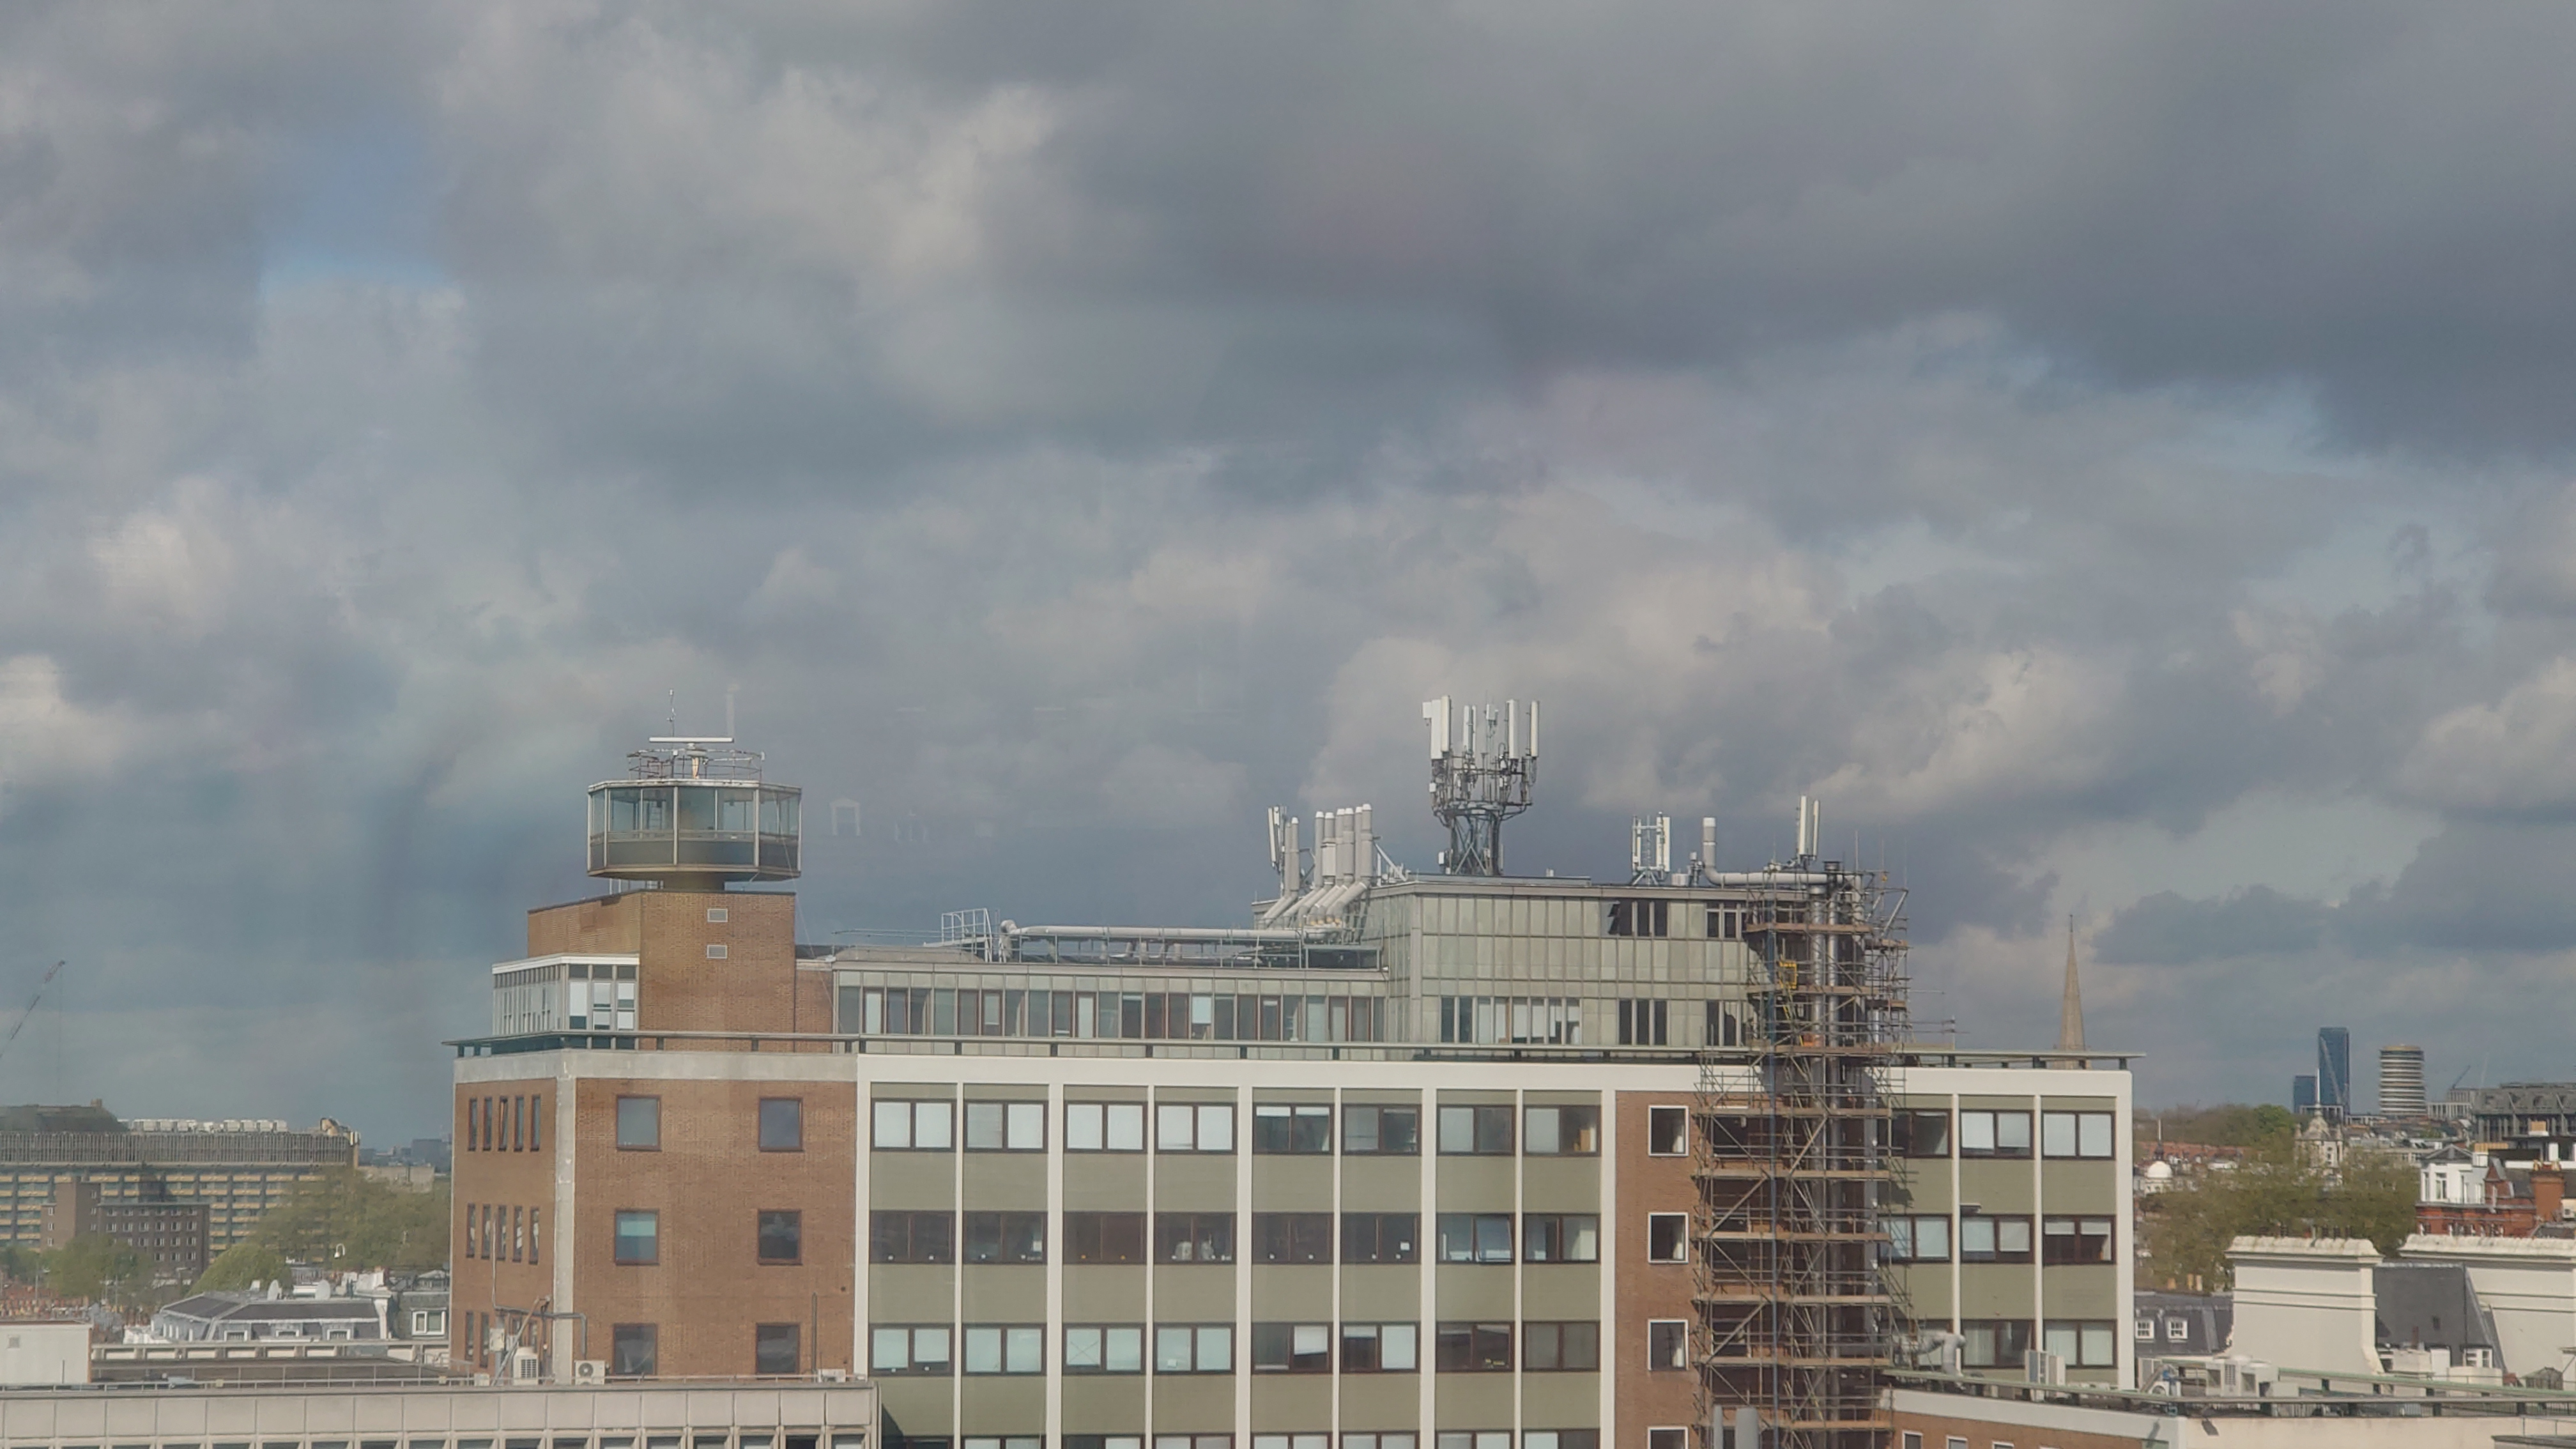
\includegraphics{../assets/viva/massive_mimo.jpg}
					}
				}
				\subfloat[Cellular statistics]{
					\resizebox{!}{3cm}{
						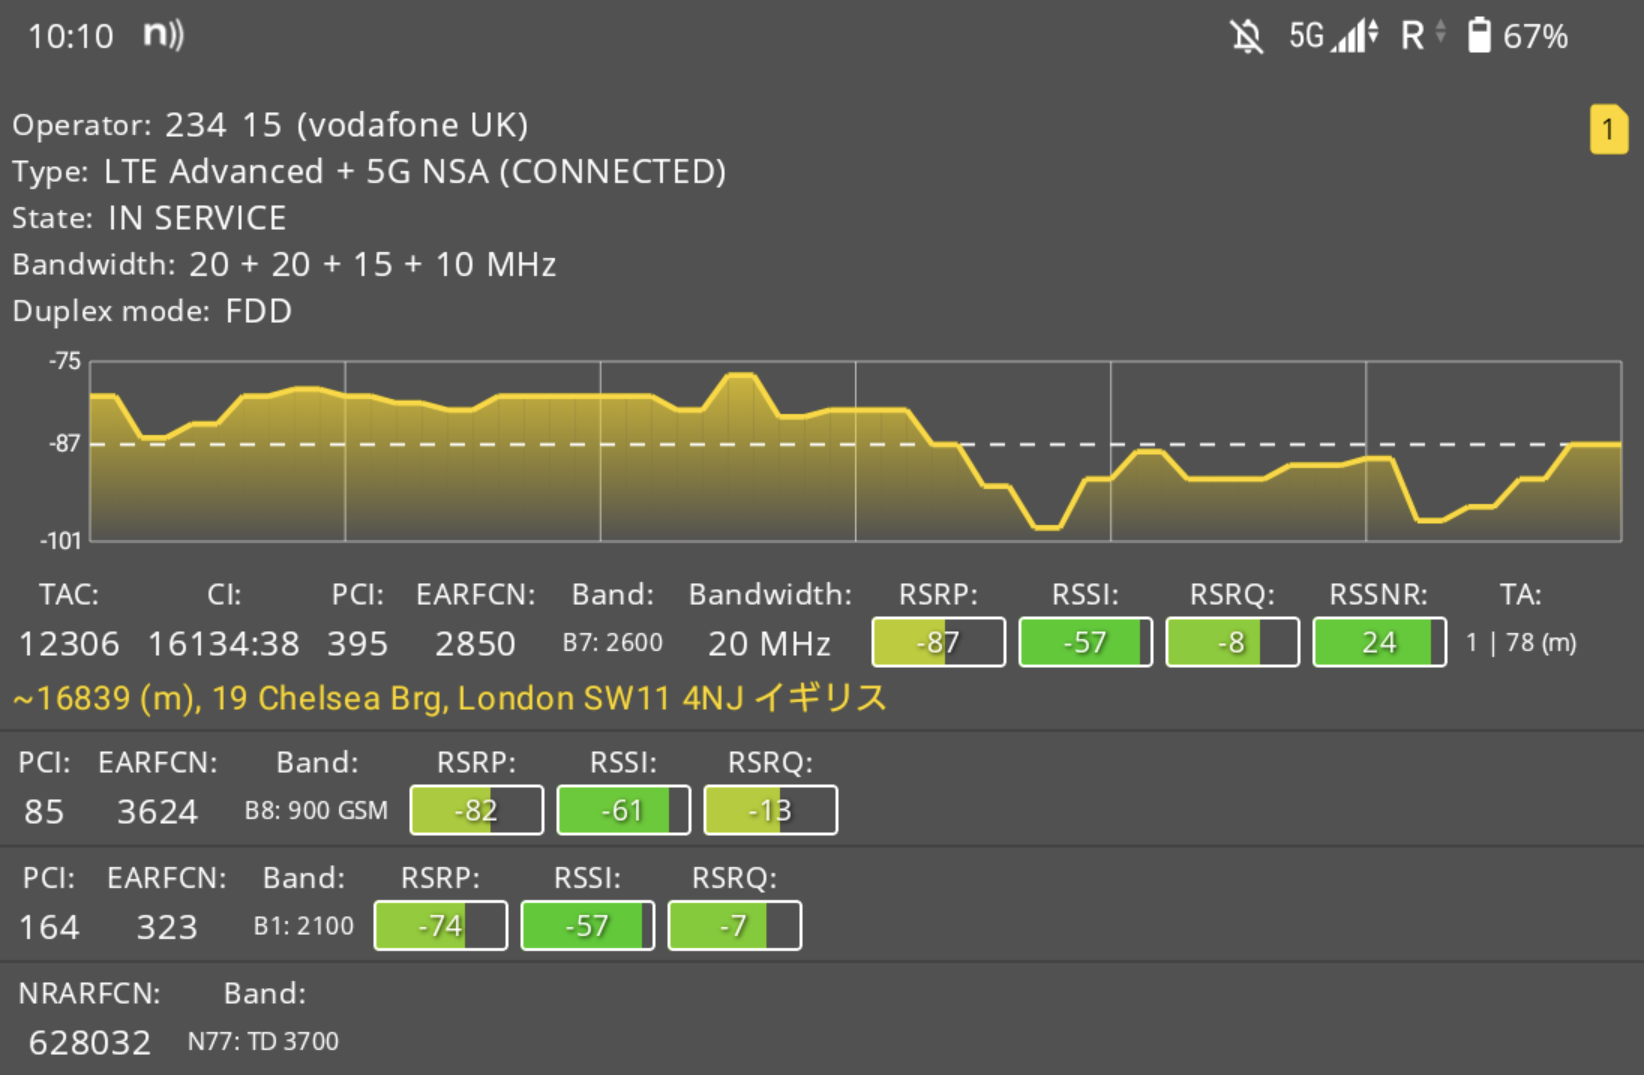
\includegraphics{../assets/viva/cellular_analysis.png}
					}
				}
			\end{figure}
		\end{block}
		\begin{block}{How far are we from the Shannon capacity?}
			\begin{equation*}
				C(\mathbf{H}) = \max_{\mathbf{Q} \succeq 0, \mathrm{tr}(\mathbf{Q}) \le P} \log \det \left( \mathbf{I} + \rho \mathbf{H} \mathbf{Q} \mathbf{H}^\mathsf{H} \right)
			\end{equation*}
			\vspace{-1em}
			\begin{itemize}
				\item Modulation, coding, and beamforming to \textcolor{gray}{adapt to} the stochastic channel
				\item \gls{ris} can \textcolor{blue}{shape and control} the channel
			\end{itemize}
		\end{block}
	\end{frame}

	\begin{frame}{What is \glsfmtshort{ris}?}
		A planar surface of controllable scattering elements for signal amplitude and phase manipulation \cite{Wu2020}.
		\begin{figure}
			\centering
			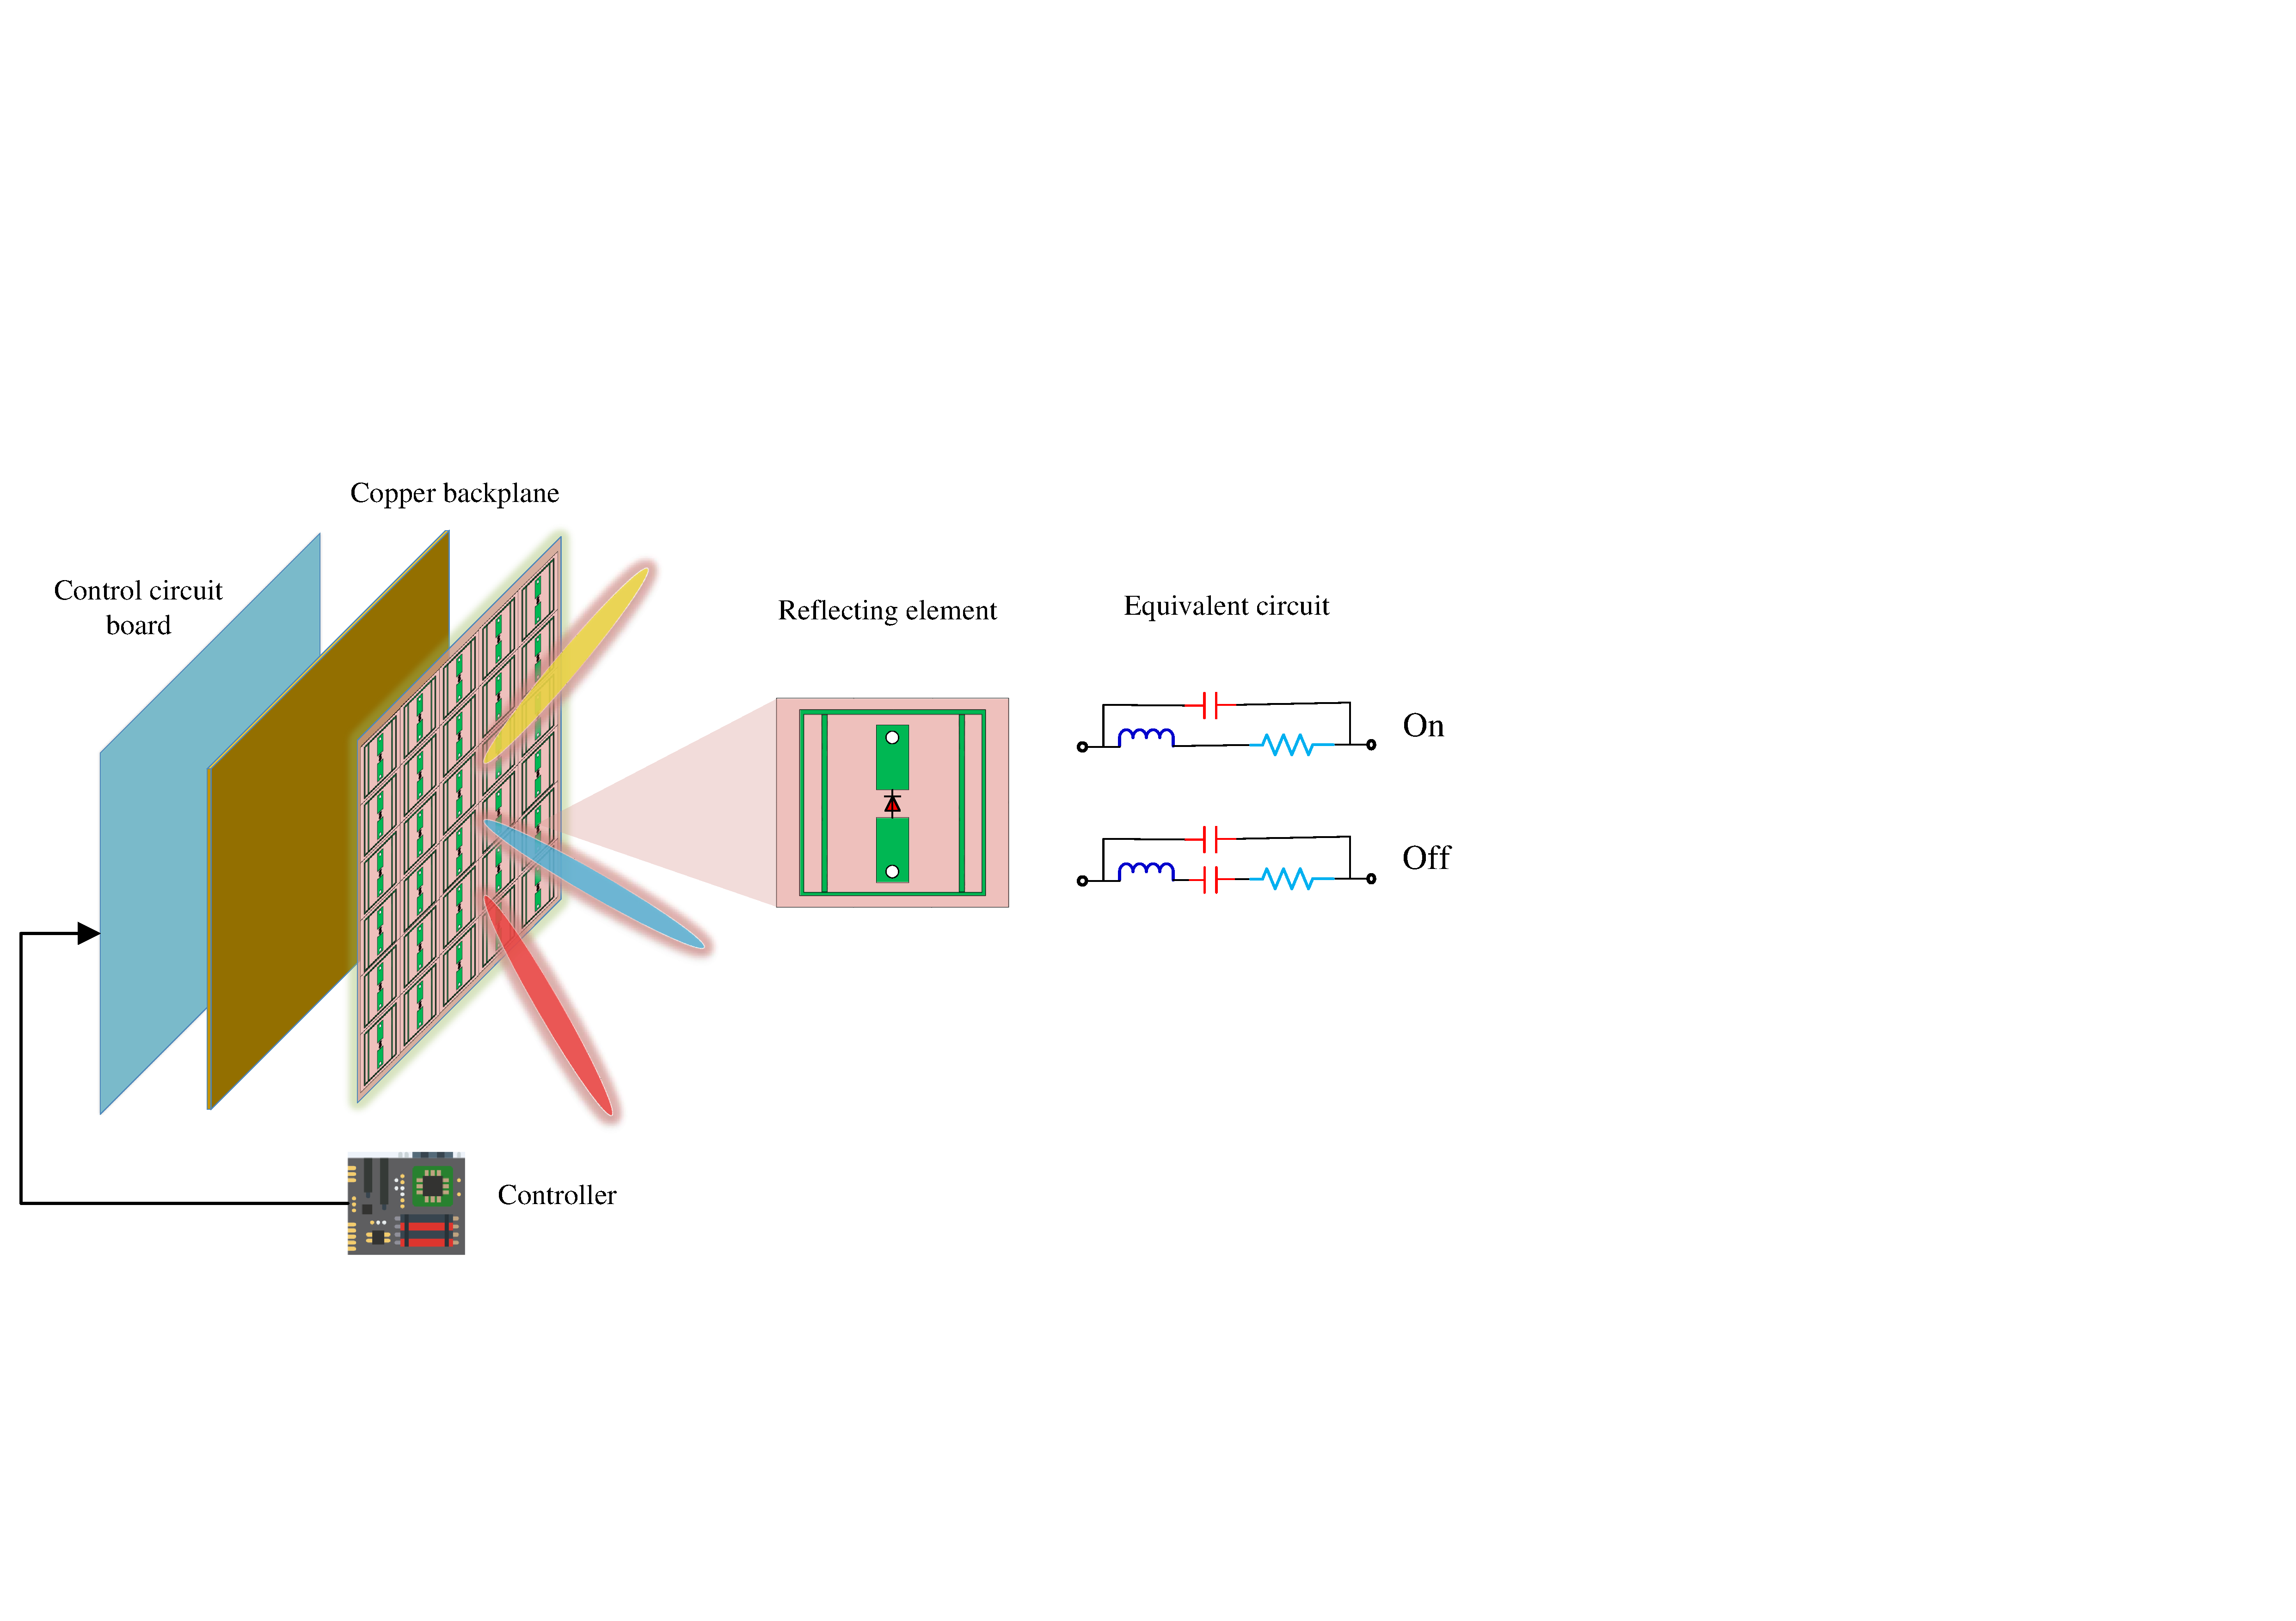
\includegraphics[width=0.65\textwidth]{../assets/viva/ris_architecture.pdf}
			\label{fg:ris_architecture}
		\end{figure}
		\begin{block}{Characteristics}
			\begin{itemize}
				\item Low-power and low-cost
				\item Negligible noise and latency
				\item Full-duplex without self-interference
				\item Programmable in real-time
			\end{itemize}
		\end{block}
	\end{frame}

	\begin{frame}{Use cases of \glsfmtshort{ris}}
		\begin{itemize}
			\item \textcolor{blue}{Beamforming} of \gls{ris} and transceiver can be jointly designed for a specific performance measure.
			\item \gls{ris} can be used for backscatter \textcolor{blue}{modulation} by periodically switching the reflection pattern.
			\item \textcolor{blue}{Channel shaping} exploits the \gls{ris} as a stand-alone device to modify the inherent properties of the propagation environment.
		\end{itemize}

		\begin{figure}
			\centering
			\subfloat[Beamforming \cite{Wu2020}]{
				\resizebox{0.32\textwidth}{!}{
					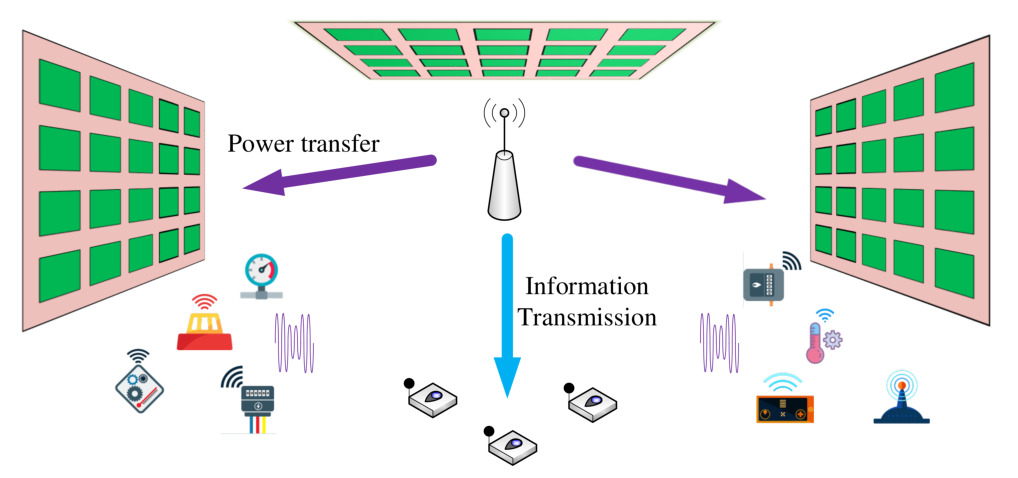
\includegraphics{../assets/viva/ris_beamforming_swipt.jpg}
				}
			}
			\subfloat[Modulation \cite{Hu2021a}]{
				\resizebox{0.32\textwidth}{!}{
					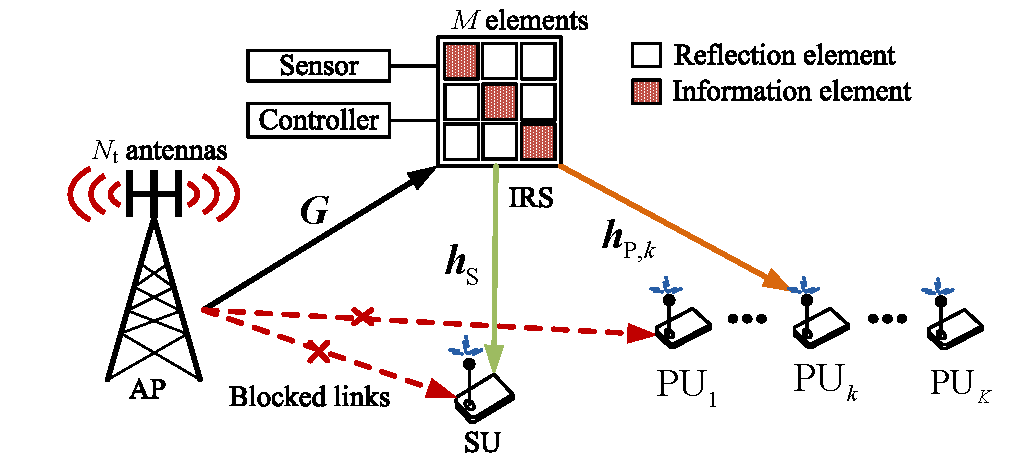
\includegraphics{../assets/viva/ris_modulation.pdf}
				}
			}
			\subfloat[Channel shaping \cite{Arslan2022}]{
				\resizebox{0.32\textwidth}{!}{
					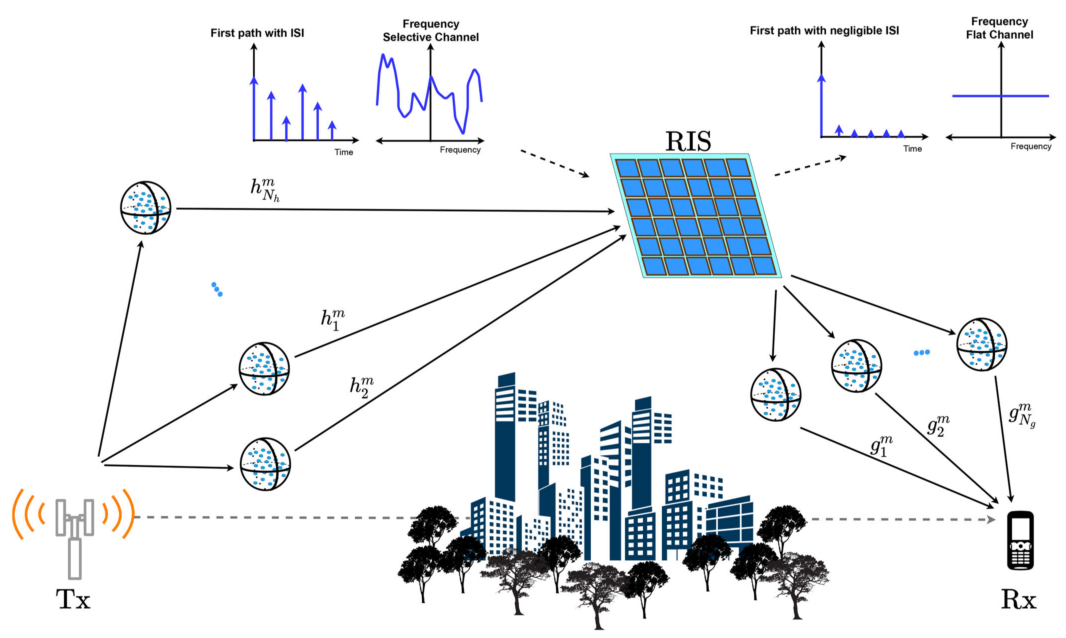
\includegraphics{../assets/viva/ris_shaping.pdf}
				}
			}
		\end{figure}
	\end{frame}
\end{section}

\begin{section}{Beamforming: \glsfmtshort{ris}-Aided \glsfmtshort{swipt}}
	\begin{frame}{\glsfmtshort{ris}-aided \glsfmtshort{swipt}: Joint waveform and beamforming design}
		\begin{block}{Overview}
			\begin{itemize}\setlength\itemsep{20pt}
				\item \textit{What does this paper propose?}

				A single-user multi-carrier \gls{swipt} system aided by a passive \gls{ris}.
				\item \textit{How does it differ from previous work?}

				We consider waveform and beamforming design for practical receiver architectures under non-linear harvester and frequency-flat \gls{ris} models.
				\item \textit{What are the benefits?}

				It exploits the spatial-frequency domain and rectifier behavior to enlarge the \gls{r-e} region, achieving squared asymptotic performance than conventional designs.
			\end{itemize}
		\end{block}
	\end{frame}

	\begin{frame}{From received signal to harvested power}
		The rectenna efficiency $\eta_3$ depends on its input waveform (power and shape).
		\begin{block}{Rectenna model}
			\begin{itemize}
				\item Linear region (constant $\eta_3$): $P_{\mathrm{DC}}^\mathrm{R} = \eta_3 P_\mathrm{RF}^\mathrm{R} = \eta_3 \mathbb{A}\bigl\{ \lvert y(t) \rvert^2 \bigr\}$
				\item Non-linear region: Taylor expansion on diode characteristic equation
				\vspace{-0.25cm}
				\begin{equation*}
					\arg_{x(t)} \max P_{\mathrm{DC}}^\mathrm{R} = \arg_{x(t)} \max z \triangleq \sum_{i=2,\text{even}}^{n_0} \beta_i \mathbb{A}\bigl\{ y^i(t) \bigr\},
					\vspace{-0.5cm}
				\end{equation*}
				where $\beta_i = I_\mathrm{S} \frac{R_\mathrm{A}^{i/2}}{i!(n v_\mathrm{T})^i}$ is a constant and $n_0$ is the truncation order.
			\end{itemize}
		\end{block}
		\begin{alertblock}{In multi-carrier \glsfmtshort{wpt} \textellipsis}
			\begin{itemize}
				\item $n_0 \ge 4$ allows components to compensate each other for higher \glsfmtshort{dc} power
				\item High \gls{papr} (e.g., multi-sine) is preferred \cite{Trotter2009}
			\end{itemize}
			\vspace{-0.5cm}
			\begin{figure}
				\centering
				\subfloat{
					\resizebox{!}{2.5cm}{
						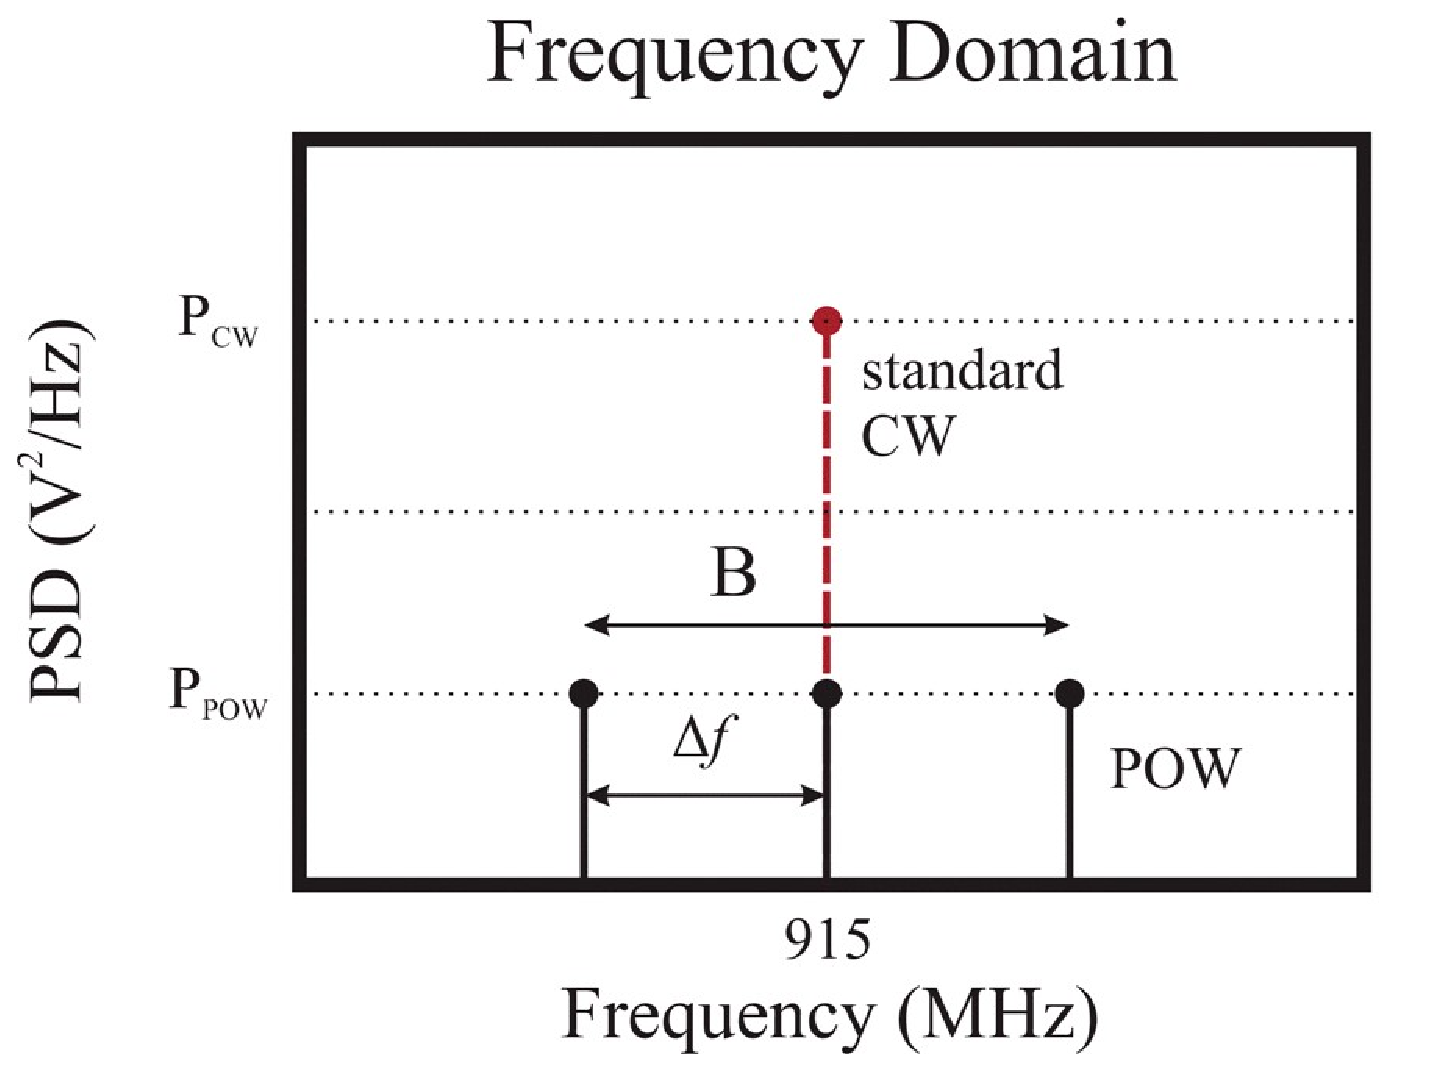
\includegraphics{../assets/viva/multisine_frequency_domain.eps}
					}
				}
				\subfloat{
					\resizebox{!}{2.5cm}{
						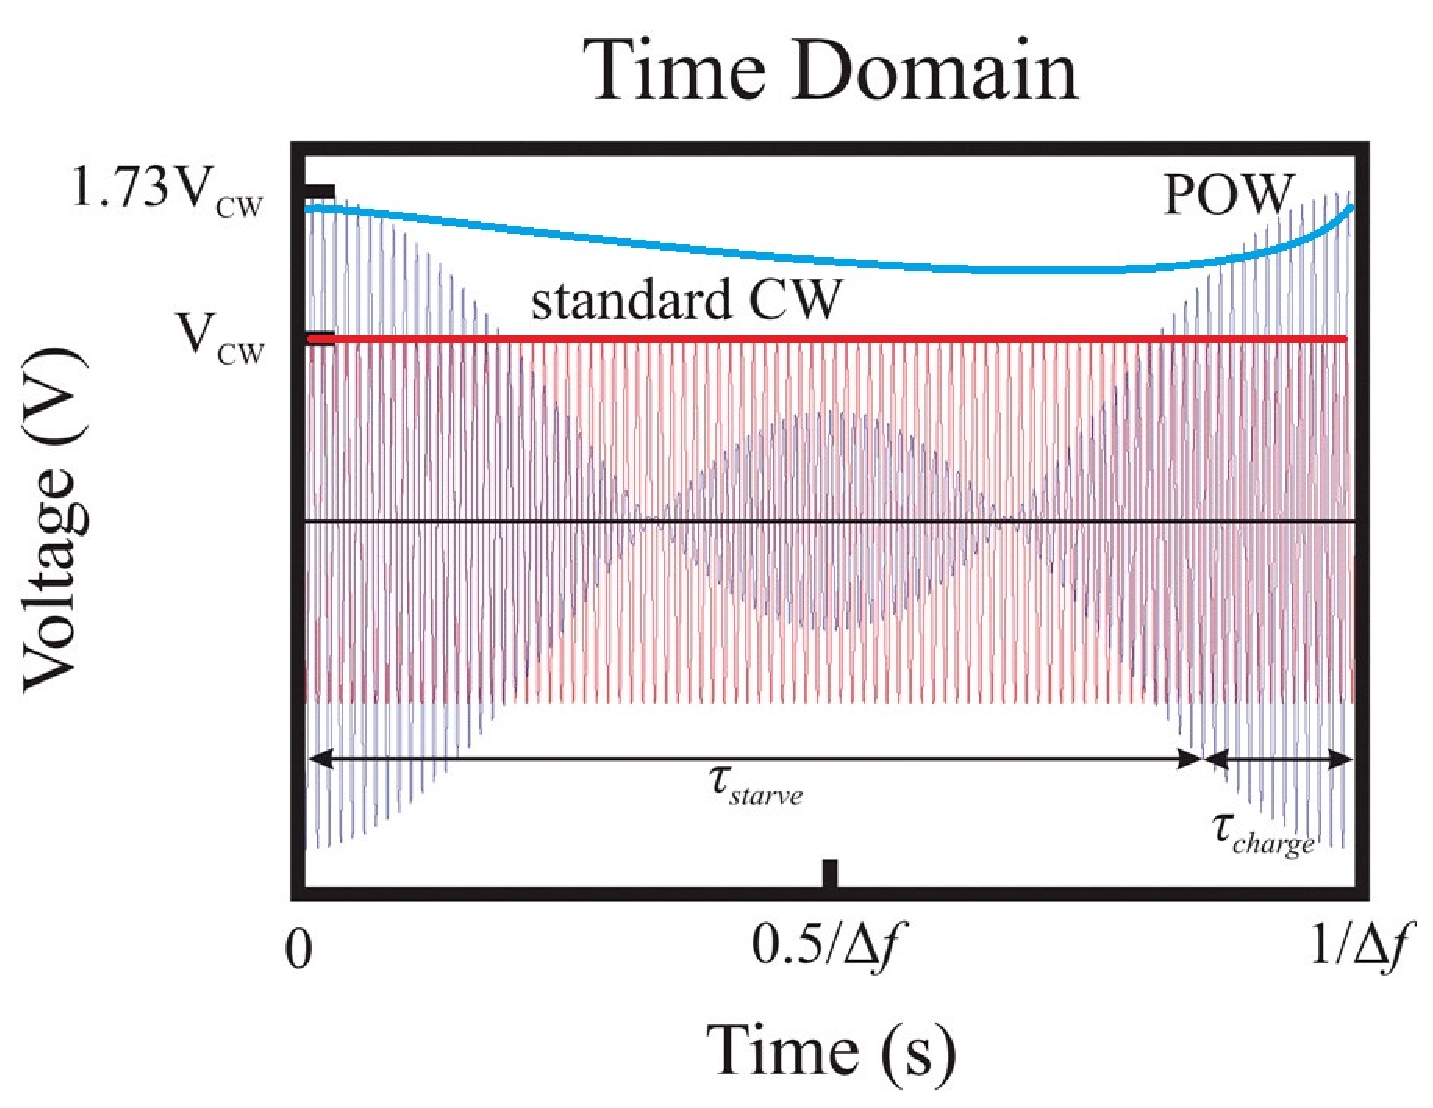
\includegraphics{../assets/viva/multisine_time_domain.eps}
					}
				}
			\end{figure}
		\end{alertblock}
	\end{frame}

	\begin{frame}{From \glsfmtshort{wpt} to \gls{ris}-aided \glsfmtshort{swipt}}
		\begin{figure}[H]
			\centering
			\def\svgwidth{0.3\columnwidth}
			\input{../assets/viva/system.eps_tex}
		\end{figure}

		\begin{itemize}
			\item \gls{swipt} features shared signal, spectrum, and infrastructure
			\item \gls{ris} enhances the RF-to-RF efficiency $\eta_2$ which has been a major concern
		\end{itemize}
		\begin{block}{Transmit waveform}
			\begin{equation*}
				\mathbf{x}(t) = \Re \left\{\sum_{n=1}^N \Bigl(\mathbf{w}_{\mathrm{I},n} \cdot \underbrace{\tilde{x}_{\mathrm{I},n}(t) e^{\jmath 2{\pi}{f_n}{t}}}_\text{modulated}+\mathbf{w}_{\mathrm{P},n} \cdot \underbrace{e^{\jmath 2{\pi}{f_n}{t}}}_\text{multi-sine}\Bigr) \right\}
			\end{equation*}
		\end{block}
		\begin{block}{Receiver architectures}
			\vspace{-0.5cm}
			\begin{figure}
				\centering
				\subfloat[\gls{ts} receiver]{
					\resizebox{0.35\columnwidth}{!}{
						\begin{circuitikz}[transform shape,align=center]
	\draw (0,0) node[bareRXantenna](r){Rx}(r.center)
		to[short] ++(0,-1) node[below]{Time switcher}
		to[short] node[spdt,anchor=in](s){} ++(0.5,0);

	\draw (s.out 1)
		to ++(1.25,0)
		to ++(0,0.5)
		to ++(1,0) node[draw,minimum width=2.5cm,anchor=west](eh){Energy\\harvester};
	% \draw (eh.east) to ++(1,0) node[draw,anchor=west,minimum width=2.5cm]{Power\\management};

	\draw (s.out 2)
		to ++(1.25,0)
		to ++(0,-0.5)
		to ++(1,0) node[draw,anchor=west,minimum width=2.5cm]{Information\\decoder};
\end{circuitikz}

% \begin{circuitikz}[transform shape,align=center]
% 	\draw (0,0) node[bareRXantenna](r){Rx}(r.center)
% 		to[short] ++(0,-1)
% 		to node[coupler,anchor=left up](c){Power splitter} ++(1,0);
% 	\draw (c.right up)
% 		to[short] ++(0.5,0)
% 		to ++(0,0.5)
% 		to ++(1,0) node[draw,minimum width=2.5cm,anchor=west](eh){Energy\\harvester};
% 	\draw (eh.east) to ++(1,0) node[draw,anchor=west,minimum width=2.5cm]{Power\\management};
% 	\draw (c.right down)
% 		to[short] ++(0.5,0)
% 		to ++(0,-0.5)
% 		to ++(1,0) node[draw,anchor=west,minimum width=2.5cm]{Information\\decoder};
% \end{circuitikz}

					}
					\label{fg:receiver_ts}
				}
				\subfloat[\gls{ps} receiver]{
					\resizebox{0.35\columnwidth}{!}{
						\begin{circuitikz}[transform shape,align=center]
	\draw (0,0) node[bareRXantenna](r){Rx}(r.center)
		to[short] ++(0,-1)
		to node[coupler,anchor=left up](c){Power splitter} ++(1,0);
	\draw (c.right up)
		to[short] ++(0.5,0)
		to ++(0,0.5)
		to ++(1,0) node[draw,minimum width=2.5cm,anchor=west](eh){Energy\\harvester};
	% \draw (eh.east) to ++(1,0) node[draw,anchor=west,minimum width=2.5cm]{Power\\management};
	\draw (c.right down)
		to[short] ++(0.5,0)
		to ++(0,-0.5)
		to ++(1,0) node[draw,anchor=west,minimum width=2.5cm]{Information\\decoder};
\end{circuitikz}

					}
					\label{fg:receiver_ps}
				}
			\end{figure}
		\end{block}
	\end{frame}

	\begin{frame}{Joint waveform and beamforming design}
		\begin{block}{Problem formulation}
			\vspace{-0.25cm}
			\begin{maxi*}
				{\scriptstyle{\boldsymbol{\theta},\mathbf{W}_\mathrm{I},\mathbf{W}_\mathrm{P},\rho}}{z(\boldsymbol{\theta},\mathbf{W}_\mathrm{I},\mathbf{W}_\mathrm{P},\rho)}{}{}
				\addConstraint{\lVert{\mathbf{W}_{\mathrm{I}}}\rVert _\mathrm{F}^2/2 + \lVert{\mathbf{W}_{\mathrm{P}}}\rVert _\mathrm{F}^2/2\le{P}}
				\addConstraint{R(\boldsymbol{\theta},\mathbf{W}_\mathrm{I},\rho) \ge \bar{R}}
				\addConstraint{\lvert{\phi_l}\rvert=1, \quad l=1,\dots,L}
				\addConstraint{0 \le \rho \le 1,}
			\end{maxi*}
		\end{block}
		\begin{exampleblock}{Solution by \glsfmtfull{bcd}}
			\begin{itemize}
				\item Optimally decouple the spatial and frequency domain design
				\begin{equation*}
					\mathbf{w}_{\mathrm{I/P}, n} = \underbrace{s_{\mathrm{I/P}, n}}_\text{frequency} \underbrace{\mathbf{p}_{\mathrm{I/P}, n}}_\text{spatial}
				\end{equation*}
				\item Active beamforming $\mathbf{p}$: \gls{mrt}
				\item Passive beamforming $\boldsymbol{\theta}$: \gls{sca}
				\item Power allocation $\mathbf{s}$ and splitting ratio $\rho$: \gls{gp}
			\end{itemize}
		\end{exampleblock}
	\end{frame}

	\begin{frame}{Simulation results: Asymptotic behavior}
		\begin{figure}
			\centering
			\subfloat[Number of transmit antennas $M$]{
				\resizebox{0.45\columnwidth}{!}{
					% This file was created by matlab2tikz.
%
%The latest updates can be retrieved from
%  http://www.mathworks.com/matlabcentral/fileexchange/22022-matlab2tikz-matlab2tikz
%where you can also make suggestions and rate matlab2tikz.
%
\definecolor{mycolor1}{rgb}{0.00000,0.44700,0.74100}%
\definecolor{mycolor2}{rgb}{0.85000,0.32500,0.09800}%
\definecolor{mycolor3}{rgb}{0.92900,0.69400,0.12500}%
%
\begin{tikzpicture}

\begin{axis}[%
width=4.036in,
height=1.531in,
at={(0.677in,2.323in)},
scale only axis,
xmin=1,
xmax=20,
xtick={ 1,  2,  4,  6,  8, 10, 12, 14, 16, 18, 20},
ymin=25,
ymax=35,
ylabel style={font=\color{white!15!black}},
ylabel={SNR [dB]},
axis background/.style={fill=white},
xmajorgrids,
ymajorgrids,
legend style={at={(0.97,0.03)}, anchor=south east, legend cell align=left, align=left, draw=white!15!black},
title style={font=\Large}, label style={font=\Large}, ticklabel style={font=\Large}, legend style={font=\Large}
]
\addplot [color=mycolor1, line width=2.0pt, mark=o, mark options={solid, mycolor1}]
  table[row sep=crcr]{%
1	25.4114090912701\\
2	27.2380228951407\\
3	28.1806581890125\\
4	29.0579705445501\\
5	29.4765358391588\\
6	30.1378186907448\\
7	30.679947158175\\
8	31.1807109572709\\
9	31.4989826016408\\
10	31.9754948092231\\
11	32.2100547605094\\
12	32.4793684081158\\
13	32.6017479139679\\
14	33.0455806994505\\
15	33.2977363152879\\
16	33.3793608838988\\
17	33.6454245558489\\
18	33.8188574644109\\
19	34.0296394451643\\
20	34.2013611372363\\
};
\addlegendentry{WF}

\end{axis}

\begin{axis}[%
width=4.036in,
height=1.531in,
at={(0.677in,0.472in)},
scale only axis,
xmin=1,
xmax=20,
xtick={ 1,  2,  4,  6,  8, 10, 12, 14, 16, 18, 20},
xlabel style={font=\color{white!15!black}},
xlabel={Number of transmit antennas},
ymin=-80,
ymax=-20,
ytick={-100,  -80,  -60,  -40,  -20,    0},
ylabel style={font=\color{white!15!black}},
ylabel={DC [dBA]},
axis background/.style={fill=white},
xmajorgrids,
ymajorgrids,
legend style={at={(0.97,0.03)}, anchor=south east, legend columns=3, legend cell align=left, align=left, draw=white!15!black},
title style={font=\Large}, label style={font=\Large}, ticklabel style={font=\Large}, legend style={font=\Large}
]
\addplot [color=mycolor1, line width=2.0pt, mark=o, mark options={solid, mycolor1}]
  table[row sep=crcr]{%
1	-72.1640311093757\\
2	-66.5715790324143\\
3	-63.3793292727081\\
4	-60.7012754464437\\
5	-59.266736864924\\
6	-57.0166388749873\\
7	-54.9404042138719\\
8	-53.2358069540989\\
9	-52.1931096939026\\
10	-50.5402642920901\\
11	-49.7737174862002\\
12	-48.6942616044043\\
13	-48.3135677149876\\
14	-46.6070871056972\\
15	-45.6179653081741\\
16	-45.4483986121797\\
17	-44.4091788705729\\
18	-43.8308588242839\\
19	-43.0166726001883\\
20	-42.3720905877998\\
};
\addlegendentry{LEH}

\addplot [color=mycolor2, dashed, line width=2.0pt, mark=+, mark options={solid, mycolor2}]
  table[row sep=crcr]{%
1	-54.8293278493535\\
2	-48.5800689706095\\
3	-45.0342330744972\\
4	-42.1572086079209\\
5	-40.5379337462381\\
6	-38.1993090160679\\
7	-35.9990333153406\\
8	-34.1537239955202\\
9	-33.0868304064636\\
10	-31.3112830269043\\
11	-30.4678953855246\\
12	-29.3603051671117\\
13	-28.9604248289287\\
14	-27.1704462396604\\
15	-26.214120462541\\
16	-25.9957086131491\\
17	-24.9246434665737\\
18	-24.2341851437915\\
19	-23.3987911541966\\
20	-22.801745202018\\
};
\addlegendentry{SMF}

\addplot [color=mycolor3, dotted, line width=2.0pt, mark=square, mark options={solid, mycolor3}]
  table[row sep=crcr]{%
1	-54.5941100581416\\
2	-48.3398061448139\\
3	-44.7929632074622\\
4	-41.9150112843405\\
5	-40.2926274936065\\
6	-37.9552739674627\\
7	-35.7534247682157\\
8	-33.9090703270243\\
9	-32.8415639562783\\
10	-31.0633765548807\\
11	-30.2229596446913\\
12	-29.1126774801063\\
13	-28.7130714340961\\
14	-26.9231116749848\\
15	-25.96807932327\\
16	-25.7475053662042\\
17	-24.6769859070682\\
18	-23.9860131480335\\
19	-23.1509323056183\\
20	-22.553989067624\\
};
\addlegendentry{GP}

\end{axis}
\end{tikzpicture}%

				}
			}
			\subfloat[Number of \gls{ris} elements $L$]{
				\resizebox{0.45\columnwidth}{!}{
					% This file was created by matlab2tikz.
%
%The latest updates can be retrieved from
%  http://www.mathworks.com/matlabcentral/fileexchange/22022-matlab2tikz-matlab2tikz
%where you can also make suggestions and rate matlab2tikz.
%
\definecolor{mycolor1}{rgb}{0.00000,0.44700,0.74100}%
\definecolor{mycolor2}{rgb}{0.85000,0.32500,0.09800}%
\definecolor{mycolor3}{rgb}{0.92900,0.69400,0.12500}%
%
\begin{tikzpicture}

\begin{axis}[%
width=4.036in,
height=1.531in,
at={(0.677in,2.323in)},
scale only axis,
xmin=1,
xmax=100,
xtick={  1,  10,  20,  30,  40,  50,  60,  70,  80,  90, 100},
ymin=16.5555734490246,
ymax=40,
ylabel style={font=\color{white!15!black}},
ylabel={SNR [dB]},
axis background/.style={fill=white},
xmajorgrids,
ymajorgrids,
legend style={at={(0.97,0.03)}, anchor=south east, legend cell align=left, align=left, draw=white!15!black},
title style={font=\huge}, label style={font=\huge}, ticklabel style={font=\LARGE}, legend style={font=\LARGE}
]
\addplot [color=mycolor1, line width=2.0pt, mark=o, mark options={solid, mycolor1}]
  table[row sep=crcr]{%
1	16.5555734490246\\
5	19.6335595133498\\
10	21.8178579734798\\
15	23.5761671596729\\
20	25.1046157566153\\
25	26.4353009128835\\
30	27.3687767493369\\
35	28.5000247501475\\
40	29.55470011095\\
45	30.2660500078313\\
50	30.8940169652101\\
55	31.7135354369005\\
60	32.341170905938\\
65	32.8036703248563\\
70	33.3976115406002\\
75	33.9866791914948\\
80	34.3153022204229\\
85	34.7478623486695\\
90	35.2274340968895\\
95	35.6119521148845\\
100	35.9998760976194\\
};
\addlegendentry{WF}

\end{axis}

\begin{axis}[%
width=4.036in,
height=1.531in,
at={(0.677in,0.472in)},
scale only axis,
xmin=1,
xmax=100,
xtick={  1,  10,  20,  30,  40,  50,  60,  70,  80,  90, 100},
xlabel style={font=\color{white!15!black}},
xlabel={Number of reflectors},
ymin=-100,
ymax=0,
ytick={-100,  -80,  -60,  -40,  -20,    0},
ylabel style={font=\color{white!15!black}},
ylabel={DC [dBA]},
axis background/.style={fill=white},
xmajorgrids,
ymajorgrids,
legend style={at={(0.97,0.03)}, anchor=south east, legend columns=3, legend cell align=left, align=left, draw=white!15!black},
title style={font=\huge}, label style={font=\huge}, ticklabel style={font=\LARGE}, legend style={font=\LARGE}
]
\addplot [color=mycolor1, line width=2.0pt, mark=o, mark options={solid, mycolor1}]
  table[row sep=crcr]{%
1	-92.5536970513039\\
5	-87.4040857061315\\
10	-81.5588189562214\\
15	-76.8140292111448\\
20	-72.3119132681356\\
25	-68.7912416779769\\
30	-65.7862313987141\\
35	-62.1723146529388\\
40	-58.5241681973142\\
45	-56.2591989620605\\
50	-53.9864632003429\\
55	-50.8433722019956\\
60	-48.7348538385412\\
65	-47.0991935158248\\
70	-44.8084149592399\\
75	-42.6836629529512\\
80	-41.4931625063164\\
85	-39.8213975436717\\
90	-37.8873698523974\\
95	-36.6019945477592\\
100	-35.0270512662257\\
};
\addlegendentry{LEH}

\addplot [color=mycolor2, dashed, line width=2.0pt, mark=+, mark options={solid, mycolor2}]
  table[row sep=crcr]{%
1	-78.9404966300438\\
5	-72.8653842234958\\
10	-65.561806372763\\
15	-60.0355415823876\\
20	-55.0277956057781\\
25	-51.0918624499135\\
30	-47.829959033523\\
35	-43.8800207934611\\
40	-39.9870037432698\\
45	-37.4246355658198\\
50	-35.09156159735\\
55	-31.7254806484209\\
60	-29.6556112190413\\
65	-27.9027388534924\\
70	-25.4289617613286\\
75	-23.32558330701\\
80	-22.0667156512475\\
85	-20.3765921162739\\
90	-18.4192057525797\\
95	-16.9836370754222\\
100	-15.3684103792823\\
};
\addlegendentry{SMF}

\addplot [color=mycolor3, dotted, line width=2.0pt, mark=square, mark options={solid, mycolor3}]
  table[row sep=crcr]{%
1	-78.711551303767\\
5	-72.6351143679569\\
10	-65.3278838246729\\
15	-59.7998504435555\\
20	-54.791570853135\\
25	-50.8545605551382\\
30	-47.5929011664101\\
35	-43.6415675742364\\
40	-39.7487995240244\\
45	-37.1874794473846\\
50	-34.8530261281813\\
55	-31.4884244381754\\
60	-29.4174064918624\\
65	-27.6650993474425\\
70	-25.1913292817342\\
75	-23.0883653237371\\
80	-21.8292565432622\\
85	-20.1391870609115\\
90	-18.1812656012089\\
95	-16.7459125238822\\
100	-15.1306956073902\\
};
\addlegendentry{GP}

\end{axis}
\end{tikzpicture}%
				}
			}
		\end{figure}
		\begin{itemize}
			\item Active beamforming: array gain $M$ and harvested power order $M^2$
			\item Passive beamforming: array gain $L^2$ and harvested power order $L^4$
			\item Superlinear thanks to coherent scattering and rectifier nonlinearity
		\end{itemize}
	\end{frame}
\end{section}

\begin{section}{Modulation: RIScatter}
	\begin{frame}{RIScatter: Unifying \gls{bc} and \glsfmtshort{ris}}
		\begin{block}{Overview}
			\begin{itemize}\setlength\itemsep{20pt}
				\item \textit{What does this paper propose?}

				RIScatter --- a batteryless cognitive radio that recycles ambient signal in an adaptive and customizable manner.
				\item \textit{How does it differ from previous work?}

				Backscatter modulation and passive beamforming are seamlessly integrated from the perspective of probability distribution.
				\item \textit{What are the benefits?}

				It supports cooperative and distributed deployment, avoids complex architecture and signal processing, and can be built over legacy systems.
			\end{itemize}
		\end{block}
	\end{frame}

	\begin{frame}{Signal model}
		RIScatter renders the node input distribution as a function of information source, \gls{csi}, and priority of coexisting links.
		\begin{figure}[H]
			\centering
			\def\svgwidth{0.6\columnwidth}
			\input{../assets/viva/riscatter_network.pdf_tex}
			\label{fg:riscatter_network}
		\end{figure}
		\begin{equation*}
			y[n] = \underbrace{\Bigl(\mathbf{h}_{\text{D}}^\mathsf{H} + \sum_{k} \alpha_k \mathbf{h}_{\text{C},k}^\mathsf{H} \textcolor{orange}{x_k}\Bigr)}_{\mathbf{h}^\mathsf{H}(\textcolor{orange}{x_{\mathcal{K}}})} \mathbf{w} \textcolor{blue}{s[n]} + v[n],
		\end{equation*}
		\vspace{-0.25cm}
		\begin{block}{Properties}
			\begin{enumerate}
				\item \textcolor{blue}{Primary} and \textcolor{orange}{backscatter} symbols are superimposed by {double modulation}
				\item Backscatter signal is much weaker due to {double fading}
				\item The spreading factor (i.e., symbol period ratio $N$) is usually large
				\item Each {state} is simultaneously part of information and beamforming {codeword}
				\item Reflection pattern over time is guided by input probability distribution
			\end{enumerate}
		\end{block}
	\end{frame}

	\begin{frame}{Low-complexity receiver}
		We propose a low-complexity receiver that exploits the aforementioned properties to avoid \gls{sic}.
		\begin{figure}[!t]
			\centering
			\subfloat{
				\resizebox{0.42\linewidth}{!}{
					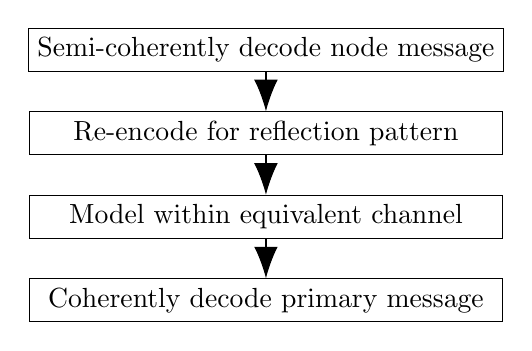
\begin{tikzpicture}[
		% every axis plot/.append style={thick},
		every node/.append style={draw,minimum width=6cm},
		align=center
	]
	\draw[-{Latex[length=4mm]}] (0,0) node[anchor=south](0){Semi-coherently decode node message} to ++(0,-0.5) node[anchor=north](1){Re-encode for reflection pattern};
	\draw[-{Latex[length=4mm]}] (1.south) to ++(0,-0.5) node[anchor=north](2){Model within equivalent channel};
	\draw[-{Latex[length=4mm]}] (2.south) to ++(0,-0.5) node[anchor=north](3){Coherently decode primary message};
\end{tikzpicture}

				}
			}
			\subfloat{
				\resizebox{0.58\linewidth}{!}{
					\definecolor{color1}{HTML}{0072BD}
\definecolor{color2}{HTML}{D95319}
\definecolor{color3}{HTML}{EDB120}
\definecolor{color4}{HTML}{7E2F8E}

\begin{tikzpicture}
	\begin{axis}[
			clip mode=individual,
			height=4cm,
			width=10cm,
			xlabel = $z$,
			ylabel = {Probability Density},
			font=\normalsize,
			no markers,
			xmin=0,
			ymin=0,
			xmax=70,
			xtick={0,12.78,20.28,29.62,70},
			xticklabels={$t_0$,$t_1$,$t_2$,$t_3$,$t_4$},
			yticklabels=\empty,
			samples = 200
		]

		\addplot+[very thick,solid,color1] gnuplot[raw gnuplot,smooth] {%
				isint(x) = (int(x)==x);
				gmm(x,rho,lambda)=rho<=0||lambda<=0?1/0:  x<0?0.0:x==0?(rho>1?0.0:rho==1?real(lambda):1/0):  exp(rho*log(lambda)+(rho-1.0)*log(x)-lgamma(rho)-lambda*x);
				set xrange [0:80];
				set yrange [0:1];
				samples=200;
				plot gmm(x,10,1)};
		\addlegendentryexpanded{$f(z \mid x_1)$}

		\addplot+[very thick,dashed,color2] gnuplot[raw gnuplot,smooth] {%
				isint(x) = (int(x)==x);
				gmm(x,rho,lambda)=rho<=0||lambda<=0?1/0:  x<0?0.0:x==0?(rho>1?0.0:rho==1?real(lambda):1/0):  exp(rho*log(lambda)+(rho-1.0)*log(x)-lgamma(rho)-lambda*x);
				set xrange [0:80];
				set yrange [0:1];
				samples=200;
				plot gmm(x,10,0.6)};
		\addlegendentryexpanded{$f(z \mid x_2)$}

		\addplot+[very thick,dotted,color3] gnuplot[raw gnuplot,smooth] {%
				isint(x) = (int(x)==x);
				gmm(x,rho,lambda)=rho<=0||lambda<=0?1/0:  x<0?0.0:x==0?(rho>1?0.0:rho==1?real(lambda):1/0):  exp(rho*log(lambda)+(rho-1.0)*log(x)-lgamma(rho)-lambda*x);
				set xrange [0:80];
				set yrange [0:1];
				samples=200;
				plot gmm(x,10,0.4)};
		\addlegendentryexpanded{$f(z \mid x_3)$}

		\addplot+[very thick,dashdotted,color4] gnuplot[raw gnuplot,smooth] {%
				isint(x) = (int(x)==x);
				gmm(x,rho,lambda)=rho<=0||lambda<=0?1/0:  x<0?0.0:x==0?(rho>1?0.0:rho==1?real(lambda):1/0):  exp(rho*log(lambda)+(rho-1.0)*log(x)-lgamma(rho)-lambda*x);
				set xrange [0:80];
				set yrange [0:1];
				samples=200;
				plot gmm(x,10,0.28)};
		\addlegendentryexpanded{$f(z \mid x_4)$}
		\draw[latex-latex] (0,0) -- (12.78,0) node[above,midway,yshift=-2]{$\mathcal{R}_1$};
		\draw[latex-latex] (12.78,0) -- (20.28,0) node[above,midway,yshift=-2]{$\mathcal{R}_2$};
		\draw[latex-latex] (20.28,0) -- (29.62,0) node[above,midway,yshift=-2]{$\mathcal{R}_3$};
		\draw[latex-latex] (29.62,0) -- (70,0) node[above,midway,yshift=-2]{$\mathcal{R}_4$};
	\end{axis}
\end{tikzpicture}

				}
			}
			\label{fg:receiver}
		\end{figure}
		\vspace{0.5cm}
		\begin{itemize}
			\item Accumulated receive energy $z=\sum_{n} \bigl\lvert y[n] \bigr\rvert^2$ follows Gamma distribution
			\item \textcolor{orange}{Backscatter detection} under primary uncertainty is part of \textcolor{blue}{channel training}
			\item Requires one energy comparison and re-encoding per backscatter symbol (much simpler than symbiotic radio with $N$ \gls{sic} and 1 combining)
		\end{itemize}
	\end{frame}

	\begin{frame}{Joint beamforming, input distribution, and energy detector design}
		\begin{block}{Problem formulation}
			\vspace{-0.25cm}
			\begin{maxi*}
				{\scriptstyle{\{\mathbf{p}_k\},\mathbf{w},\mathbf{t}}}{\rho R_\text{P} + (1-\rho) \sum\nolimits_{k} R_{\text{B},k}}{}{}
				\addConstraint{\mathbf{1}^\mathsf{T} \mathbf{p}_k=1,}{\quad \mathbf{p}_k \ge \mathbf{0},}{\quad \forall k}
				\addConstraint{t_{l-1} \le t_l,}{\quad t_l \ge 0,}{\quad \forall l}
				\addConstraint{\lVert \mathbf{w} \rVert^2 \le P,}{}{}
			\end{maxi*}
		\end{block}
		\begin{exampleblock}{Solution by \gls{bcd}}
			\begin{itemize}
				\item Input distribution $\{\mathbf{p}_k\}$: \gls{kkt}
				\item Active beamforming $\mathbf{w}$: \gls{pga}
				\item Energy decision threshold $\mathbf{t}$: \gls{dp}
			\end{itemize}
		\end{exampleblock}
	\end{frame}

	\begin{frame}{Simulation results: Input distribution and rate region}
		\begin{figure}[!t]
			\centering
			\subfloat{
				\resizebox{0.48\linewidth}{!}{
					% This file was created by matlab2tikz.
%
%The latest updates can be retrieved from
%  http://www.mathworks.com/matlabcentral/fileexchange/22022-matlab2tikz-matlab2tikz
%where you can also make suggestions and rate matlab2tikz.
%
\definecolor{mycolor1}{rgb}{0.00000,0.44706,0.74118}%
\definecolor{mycolor2}{rgb}{0.85098,0.32549,0.09804}%
\definecolor{mycolor3}{rgb}{0.92941,0.69412,0.12549}%
\definecolor{mycolor4}{rgb}{0.49412,0.18431,0.55686}%
%
\begin{tikzpicture}

\begin{axis}[%
width=4.079in,
height=1.587in,
at={(0.684in,0.361in)},
scale only axis,
xmin=1,
xmax=4,
xtick={1, 2, 3, 4},
xlabel style={font=\color{white!15!black}},
xlabel={Reflection State},
ymin=0,
ymax=1,
ytick={  0, 0.2, 0.4, 0.6, 0.8,   1},
ylabel style={font=\color{white!15!black}},
ylabel={Probability\\Distribution},
axis background/.style={fill=white},
xmajorgrids,
ymajorgrids,
legend style={at={(0.03,0.97)}, anchor=north west, legend cell align=left, align=left, draw=white!15!black},
align=center,
title style={font=\LARGE},
label style={font=\LARGE},
ticklabel style={font=\Large},
legend style={font=\Large}
]
\addplot [color=mycolor1, line width=2.0pt, mark=o, mark options={solid, mycolor1}]
  table[row sep=crcr]{%
1	6.48337921881147e-07\\
2	0.504332536970115\\
3	0.495666065268481\\
4	7.49423481629768e-07\\
};
\addlegendentry{$\rho =0$}

\addplot [color=mycolor2, dashed, line width=2.0pt, mark=+, mark options={solid, mycolor2}]
  table[row sep=crcr]{%
1	9.07520883479571e-08\\
2	0.401497967775065\\
3	0.598501822229458\\
4	1.1924338950349e-07\\
};
\addlegendentry{$\rho =0.1$}

\addplot [color=mycolor3, dotted, line width=2.0pt, mark=square, mark options={solid, mycolor3}]
  table[row sep=crcr]{%
1	5.20790909800095e-09\\
2	0.192484685585801\\
3	0.807515300031504\\
4	9.17478600370393e-09\\
};
\addlegendentry{$\rho =0.25$}

\addplot [color=mycolor4, dashdotted, line width=2.0pt, mark=x, mark options={solid, mycolor4}]
  table[row sep=crcr]{%
1	1.08446044988811e-11\\
2	8.27854203489531e-06\\
3	0.999991721175464\\
4	2.71656646770891e-10\\
};
\addlegendentry{$\rho =1$}

\end{axis}
\end{tikzpicture}%
				}
			}
			\subfloat{
				\resizebox{0.48\linewidth}{!}{
					% This file was created by matlab2tikz.
%
%The latest updates can be retrieved from
%  http://www.mathworks.com/matlabcentral/fileexchange/22022-matlab2tikz-matlab2tikz
%where you can also make suggestions and rate matlab2tikz.
%
\definecolor{mycolor1}{rgb}{0.30100,0.74500,0.93300}%
\definecolor{mycolor2}{rgb}{0.46600,0.67400,0.18800}%
\definecolor{mycolor3}{rgb}{0.49400,0.18400,0.55600}%
\definecolor{mycolor4}{rgb}{0.92900,0.69400,0.12500}%
\definecolor{mycolor5}{rgb}{0.85000,0.32500,0.09800}%
\definecolor{mycolor6}{rgb}{0.00000,0.44700,0.74100}%
%
\begin{tikzpicture}

\begin{axis}[%
	width=4.079in,
	height=3.432in,
at={(0.673in,0.356in)},
scale only axis,
xmin=0,
xmax=6.5227548374066,
xlabel style={font=\color{white!15!black}},
xlabel={Primary Rate [bits/s/Hz]},
ymin=0,
ymax=2,
ylabel style={font=\color{white!15!black}},
ylabel={Backscatter Rate [bits/BB]},
axis background/.style={fill=white},
xmajorgrids,
ymajorgrids,
legend style={at={(0.03,0.97)}, anchor=north west, legend cell align=left, align=left, draw=white!15!black},
align=center,
% title style={font=\huge},
% label style={font=\huge},
% ticklabel style={font=\LARGE},
% legend style={font=\LARGE},
reverse legend,
every axis plot/.append style={line width=2pt}
]
\addplot [color=mycolor1, line width=2.0pt, mark=triangle, mark options={solid, rotate=180, mycolor1}]
  table[row sep=crcr]{%
6.33724402501803	1.39764296268229\\
0	1.39764296268229\\
0	0\\
6.52275483678685	0\\
6.52275483678685	2.37312052924553e-08\\
6.38739454470992	1.3235811846854\\
6.35422040211439	1.38916612409166\\
6.34857862205488	1.39386686170527\\
6.3445353675389	1.39608085009443\\
6.34291602910554	1.3966977322109\\
6.34149846039129	1.39711118534274\\
6.34024731759122	1.39737797077851\\
6.3391350240222	1.3975379071887\\
6.33862394227692	1.39758701988787\\
6.33813974610465	1.39761939115801\\
6.33795313341839	1.39762818964178\\
6.33777036860279	1.39763482338317\\
6.3375913342378	1.3976394187338\\
6.33741590881855	1.39764209463684\\
6.33724402501803	1.39764296268229\\
};
\addlegendentry{RIScatter}

\addplot[only marks, mark=triangle, mark options={}, mark size=2.3570pt, draw=mycolor2] table[row sep=crcr]{%
x	y\\
6.5227548374066	0\\
};
\addlegendentry{RIS}

\addplot[only marks, mark=+, mark options={}, mark size=3.5355pt, draw=mycolor3] table[row sep=crcr]{%
x	y\\
6.34321982467796	2\\
};
\addlegendentry{SR}

\addplot[only marks, mark=x, mark options={}, mark size=3.5355pt, draw=mycolor4] table[row sep=crcr]{%
x	y\\
5.90778796357092	1.34857377961699\\
};
\addlegendentry{AmBC}

\addplot[only marks, mark=square, mark options={}, mark size=2.5000pt, draw=mycolor5] table[row sep=crcr]{%
x	y\\
0	1.99999999999997\\
};
\addlegendentry{BBC}

\addplot[only marks, mark=o, mark options={}, mark size=2.7386pt, draw=mycolor6] table[row sep=crcr]{%
x	y\\
6.34314881160129	0\\
};
\addlegendentry{Legacy}

\end{axis}
\end{tikzpicture}%

				}
			}
		\end{figure}
		\begin{itemize}
			\item Increasing $\rho$ from 0 to 1 evolves from \gls{bc} to \gls{ris}
			\item Backscatter rate is lower than \glsfmtshort{sr} (due to energy detection) but higher than \glsfmtshort{ambc} (due to adaptive encoding)
			\item Active and passive transmission can share resource with mutual benefits
			% creates a smooth transition from backscatter modulation to passive beamforming
		\end{itemize}
	\end{frame}
\end{section}

\begin{section}{Shaping: \glsfmtshort{bd}-\glsfmtshort{ris} in \glsfmtshort{mimo}}
	\begin{frame}{Channel shaping using \glsfmtshort{ris}: From diagonal model to beyond}
		\begin{block}{Overview}
			\begin{itemize}\setlength\itemsep{20pt}
				\item \textit{What does this paper study?}

				To what extent can a passive \gls{ris} redistribute the singular values of a \gls{mimo} channel.
				\item \textit{How does it differ from previous work?}

				We consider a \gls{bd} architecture, depict the singular value region, derive analytical bounds, and solve the rate maximization problem.
				\item \textit{What are the benefits?}

				Channel shaping is ubiquitous for communication, sensing, and power transfer, which helps to decouple the \gls{ris}-transceiver design.
				We also propose an efficient and universal \gls{bd}-\gls{ris} design framework.
			\end{itemize}
		\end{block}
	\end{frame}

	\begin{frame}{Wave scattering model}
		\begin{block}{Diagonal \glsfmtshort{ris}}
			Each element acts as an individual scatterer with phase shift only
			\begin{equation*}
				\mathbf{\Theta} = \mathrm{diag}(\theta_1, \ldots, \theta_{N_\mathrm{S}}) = \mathrm{diag}(e^{\jmath \phi_1}, \ldots, e^{\jmath \phi_{N_\mathrm{S}}})
				%  =
				% \begin{bsmallmatrix}
				% 	\theta_1 & 0 & \cdots & 0 \\
				% 	0 & \theta_2 & \cdots & 0 \\
				% 	\vdots & \vdots & \ddots & \vdots \\
				% 	0 & 0 & \cdots & \theta_{N_\mathrm{S}}
				% \end{bsmallmatrix}
				\label{eq:diagonal_scattering_matrix}
			\end{equation*}
		\end{block}

		\begin{block}{\glsfmtshort{bd}-\glsfmtshort{ris}}
			Each group contains $L$ connected elements, allowing amplitude and phase control
			% \vspace{-0.25cm}
			\begin{equation*}
				\mathbf{\Theta} = \mathrm{diag}(\mathbf{\Theta}_1,\ldots,\mathbf{\Theta}_G), \quad \mathbf{\Theta}_g^\mathsf{H} \mathbf{\Theta}_g = \mathbf{I}_L, \quad \forall g
				\label{eq:bd_ris}
			\end{equation*}
			\vspace{-0.5cm}
			\begin{figure}[H]
				\centering
				\resizebox{0.5\columnwidth}{!}{
					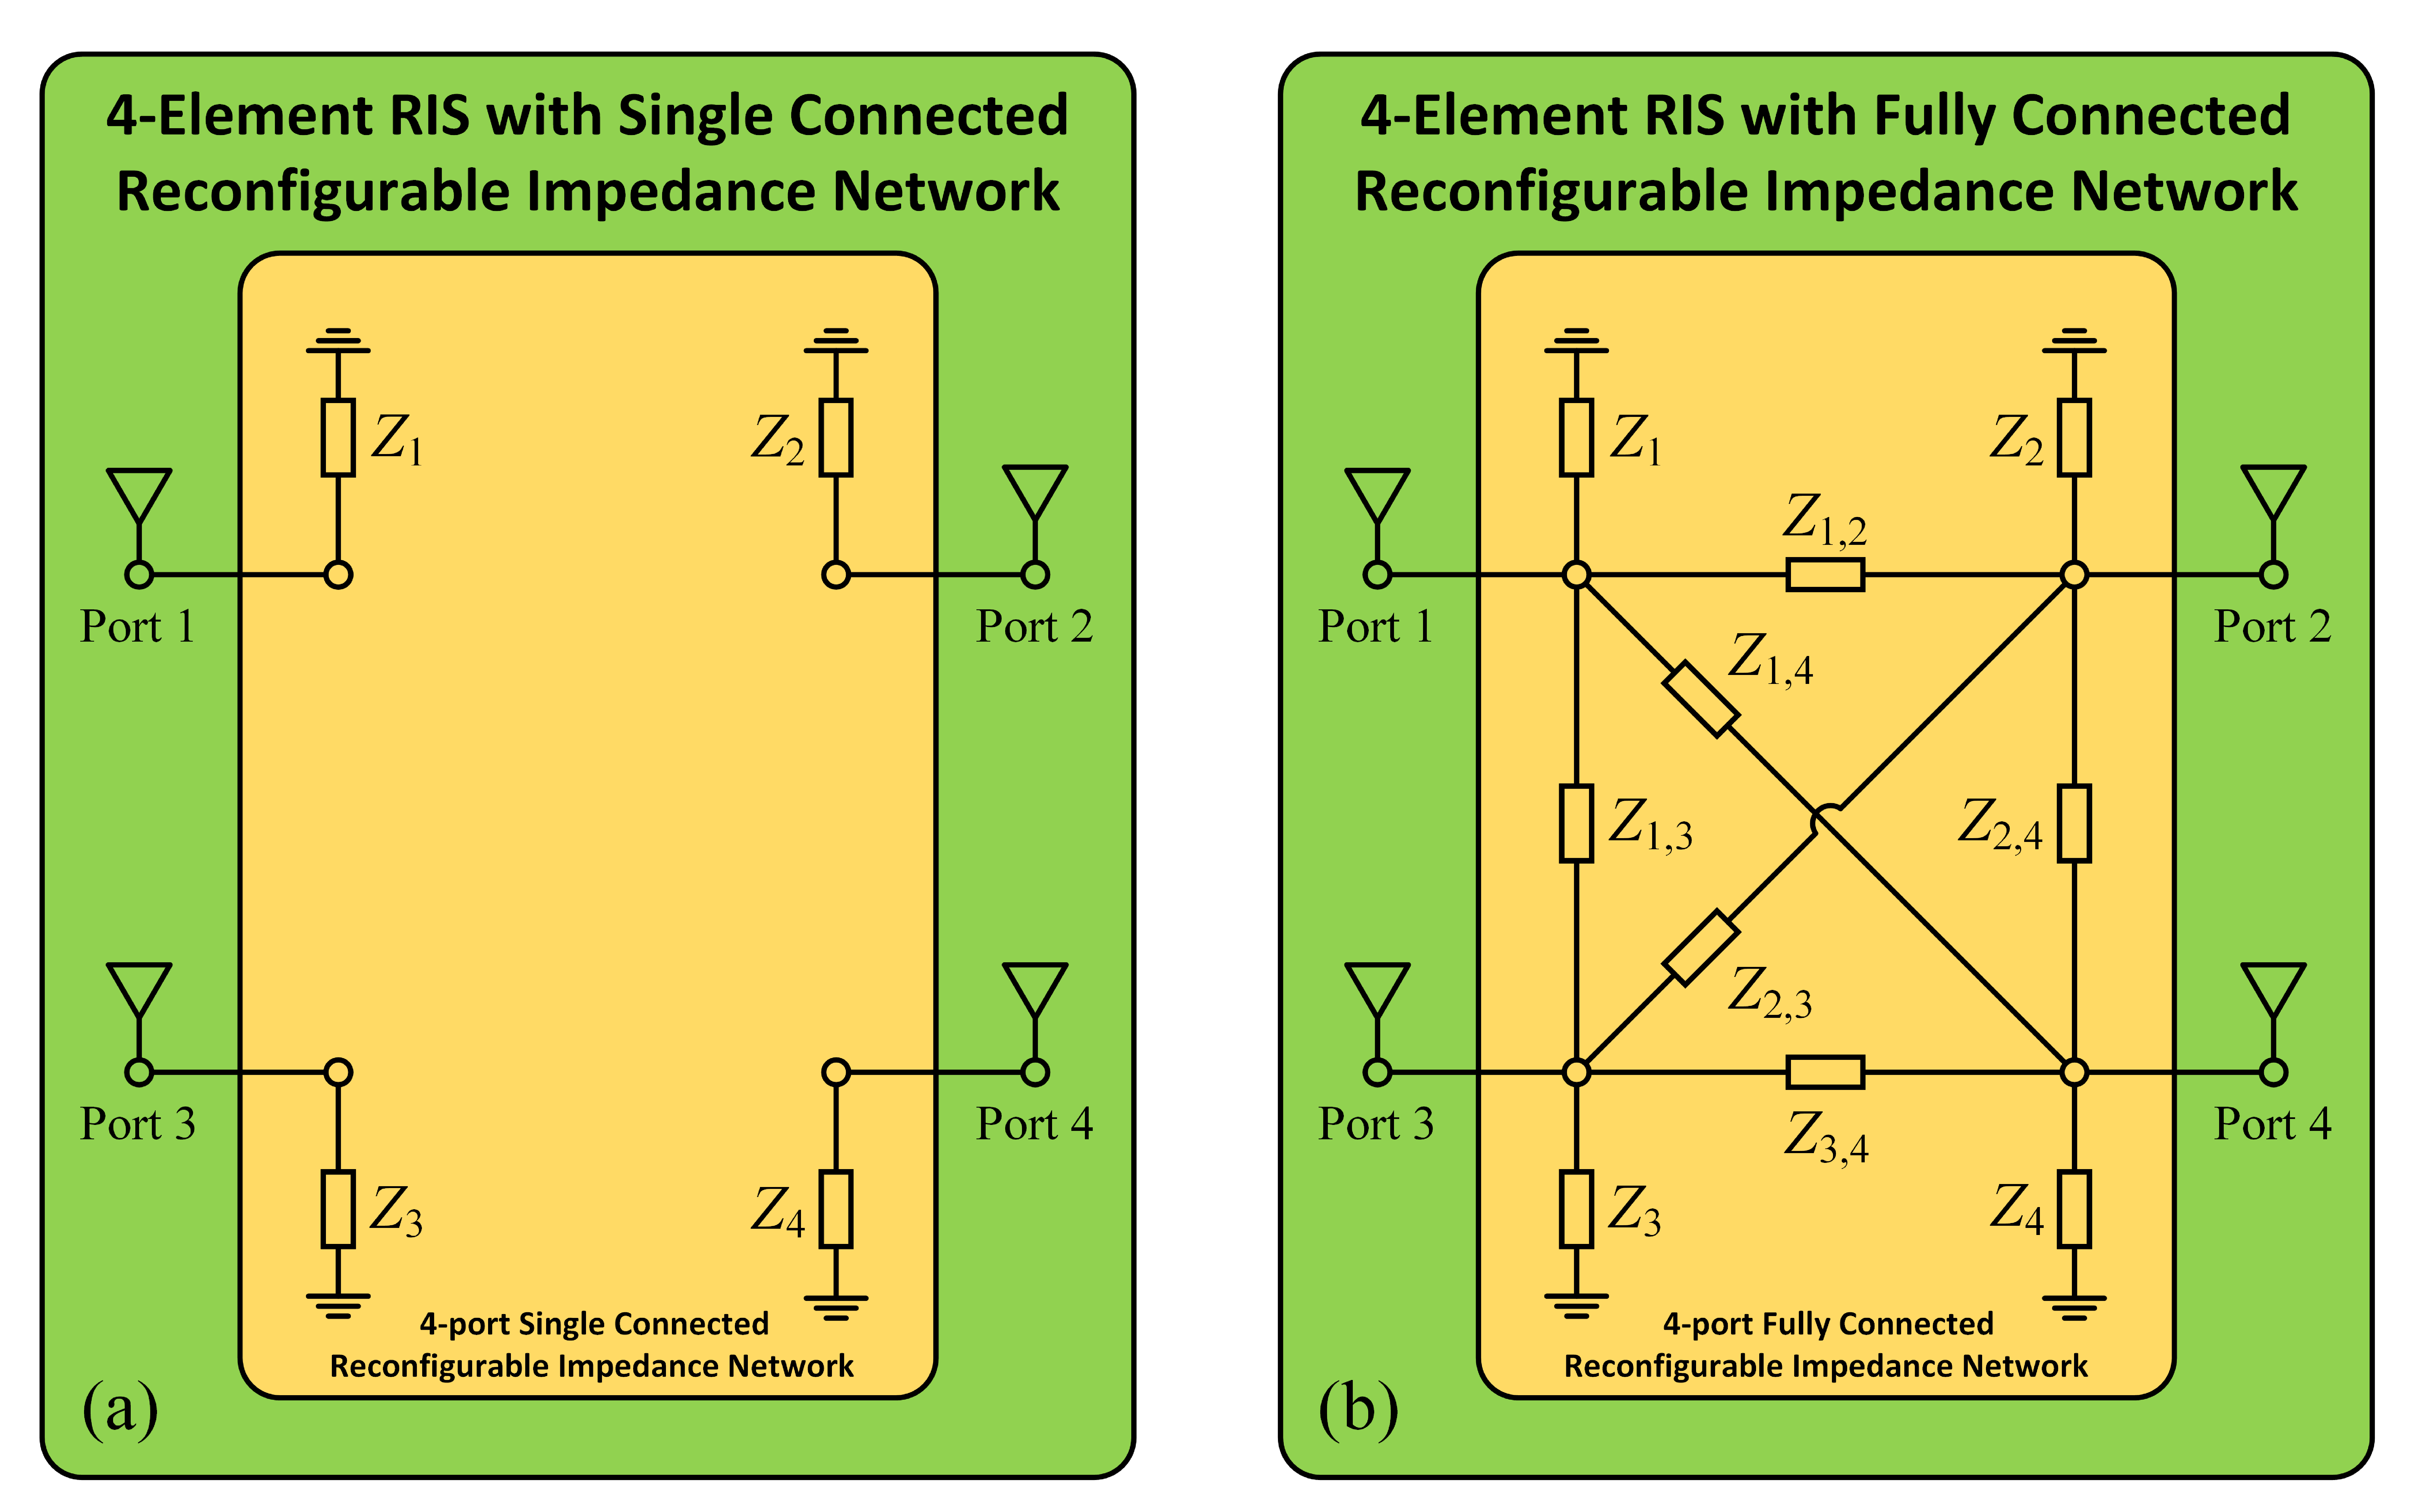
\includegraphics{../assets/viva/bd_ris_architecture_1.eps}
				}
				\caption{Architecture of diagonal and \gls{bd}-\gls{ris} \cite{Shen2020a}}
				\label{fg:bd_ris_architecture_2}
			\end{figure}

		\end{block}
	\end{frame}

	\begin{frame}{Proposed geodesic update via Lie algebra}
		\vspace{-0.25cm}
		\begin{figure}
			\centering
			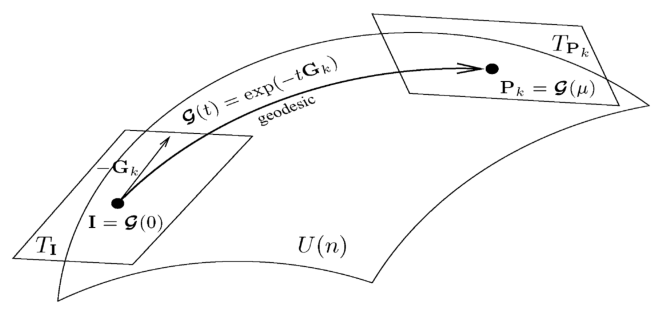
\includegraphics[width=0.5\textwidth]{../assets/viva/lie_group.pdf}
		\end{figure}
		\vspace{-0.25cm}
		\begin{block}{Non-geodesic vs geodesic \gls{rcg}}
			\begin{itemize}
				\item Non-geodesic: add then retract
				\begin{equation*}
					\bar{\mathbf{\Theta}}_g^{(r+1)} = \mathbf{\Theta}_g^{(r)} + \mu \mathbf{D}_g^{(r)}, \quad \mathbf{\Theta}_g^{(r+1)} = \bar{\mathbf{\Theta}}_g^{(r+1)} \bigl({\bar{\mathbf{\Theta}}_g^{(r+1)\mathsf{H}}} \bar{\mathbf{\Theta}}_g^{(r+1)}\bigr)^{-1/2}
				\end{equation*}
				\item Geodesic: multiplicative and rotational update
				\begin{equation*}
					\mathbf{\Theta}_g^{(r+1)} = \mathbf{G}_g^{(r)}(\mu) = \exp(\mu \mathbf{D}_g^{(r)}) \mathbf{\Theta}_g^{(r)}
					\label{eq:update_geodesic}
				\end{equation*}
			\end{itemize}
		\end{block}
		\begin{exampleblock}{Performance comparison}
			\begin{table}
				\label{tb:complexity_test}
				\centering
				\tiny
				\begin{tabular}{ccccccc}
					\toprule
					\multirow{2}{*}{\gls{rcg} path} & \multicolumn{3}{c}{$N_\mathrm{S}=16$} & \multicolumn{3}{c}{$N_\mathrm{S}=256$}                                                               \\ \cmidrule(lr){2-4} \cmidrule(lr){5-7}
													& Objective                             & Iterations                             & Time [s]         & Objective        & Iterations & Time [s] \\ \midrule
					Geodesic                        & $\num{4.359e-3}$                      & 11.59                                  & $\num{1.839e-2}$ & $\num{1.163e-2}$ & 25.58      & 3.461    \\
					Non-geodesic                    & $\num{4.329e-3}$                      & 30.92                                  & $\num{5.743e-2}$ & $\num{1.116e-2}$ & 61.40      & 13.50    \\ \bottomrule
				\end{tabular}
			\end{table}
		\end{exampleblock}
	\end{frame}

	\begin{frame}{Problem formulation}
		\begin{block}{Pareto frontier of channel singular values}
			\vspace{-0.25cm}
			\begin{maxi*}
				{\scriptstyle{\mathbf{\Theta}}}{\sum_n \rho_n \sigma_n(\mathbf{H})}{}{}
				\addConstraint{\mathbf{\Theta}_g^\mathsf{H} \mathbf{\Theta}_g=\mathbf{I},}{\quad \forall g,}{}
			\end{maxi*}
		\end{block}
		\begin{block}{Achievable rate maximization}
			\vspace{-0.25cm}
			\begin{maxi*}
				{\scriptstyle{\mathbf{W},\mathbf{\Theta}}}{R = \log \det \biggl(\mathbf{I} + \frac{\mathbf{W}^\mathsf{H}\mathbf{H}^\mathsf{H}\mathbf{H}\mathbf{W}}{\eta}\biggr)}{}{}
				\addConstraint{\lVert \mathbf{W} \rVert _\mathrm{F}^2}{\le P}
				\addConstraint{\mathbf{\Theta}_g^\mathsf{H} \mathbf{\Theta}_g}{=\mathbf{I}, \quad \forall g.}
			\end{maxi*}
		\end{block}
		\begin{exampleblock}{Solution by group-wise geodesic \glsfmtshort{rcg}}
			\begin{itemize}
				\item Faster convergence thanks to appropriate parameter space
				\item Optimal and low-complexity solutions
			\end{itemize}
		\end{exampleblock}
	\end{frame}

	\begin{frame}{Simulation results: Singular value and achievable rate}
		\begin{figure}
			\centering \hspace*{-1cm}
			\subfloat[$2 \times 32 \times 2$\label{fg:singular_pareto_sx32}]{
				\resizebox{!}{3.2cm}{
					% This file was created by matlab2tikz.
%
%The latest updates can be retrieved from
%  http://www.mathworks.com/matlabcentral/fileexchange/22022-matlab2tikz-matlab2tikz
%where you can also make suggestions and rate matlab2tikz.
%
\definecolor{mycolor1}{rgb}{0.00000,0.44706,0.74118}%
\definecolor{mycolor2}{rgb}{0.85098,0.32549,0.09804}%
\definecolor{mycolor3}{rgb}{0.92941,0.69412,0.12549}%
\definecolor{mycolor4}{rgb}{0.49412,0.18431,0.55686}%
%
\begin{tikzpicture}

\begin{axis}[%
width=7.607cm,
height=6cm,
at={(0cm,0cm)},
scale only axis,
xmin=0.000850130707459294,
xmax=0.001495567105556,
xlabel style={font=\color{white!15!black}},
xlabel={$\sigma_1(\mathbf{H})$},
ymin=5.81124124465135e-05,
ymax=0.000756440229046408,
ylabel style={font=\color{white!15!black}},
ylabel={$\sigma_2(\mathbf{H})$},
axis background/.style={fill=white},
xmajorgrids,
ymajorgrids,
legend style={at={(0.03,0.03)}, anchor=south west, legend cell align=left, align=left, draw=white!15!black},
every axis plot/.append style={line width=1.5pt}
]
\addplot[only marks, mark=triangle, mark options={}, mark size=2.3570pt, draw=black] table[row sep=crcr]{%
x	y\\
0.00117134827739843	0.000407871162732991\\
};
\addlegendentry{Direct}

\addplot [color=mycolor1, line width=2.0pt, mark=o, mark options={solid, mycolor1}]
  table[row sep=crcr]{%
0.00137955431172681	0.000588505616267897\\
0.00137418269622086	0.000593615295742653\\
0.00136749093451528	0.000599376628494274\\
0.00135890213089589	0.000606072077153129\\
0.00134973459427533	0.000612532388777538\\
0.0013410733835681	0.000618021117436472\\
0.00133234723576559	0.000622963402732477\\
0.00132298835416539	0.000627671842535913\\
0.00131283927996255	0.000632167827335414\\
0.00130175068079053	0.000636441315549385\\
0.00128938330235212	0.000640521027244044\\
0.00127272827567336	0.000645071318717164\\
0.001239223656723	0.000652826329399127\\
0.00121181294625974	0.000657515986538869\\
0.0011948709631463	0.000659612394858911\\
0.00117924446441914	0.000660770327164558\\
0.00116465364423377	0.000661132293899478\\
0.00113619330680091	0.000660369140191549\\
0.00111681335066479	0.00065893828544607\\
0.00110400776403201	0.00065738003226823\\
0.00109347165774378	0.000655554479547099\\
0.00108325459149789	0.00065326015322085\\
0.00107295870959626	0.000650409170334344\\
0.00105545417968485	0.000644538951540662\\
0.00104038763128197	0.000638729468304811\\
0.00102417401193919	0.000631551077219278\\
0.00101241548515279	0.000625650365523887\\
0.00100425860502732	0.000621064981892173\\
0.0009940831826727	0.000614742850166296\\
0.000987415602981892	0.000610234296197683\\
0.000980849676409786	0.000605333755974594\\
0.000975257972036462	0.000600727614092169\\
0.000970012018476528	0.000595952796375679\\
0.000965688097012915	0.000591642872687785\\
0.000961613627835618	0.000587170882990767\\
0.000958073981707157	0.000582866103258482\\
0.000954801020084192	0.000578430681164638\\
0.000951712819265589	0.000573772911667256\\
0.000947720748747545	0.000567031466535514\\
0.00094368967956249	0.000559421880095604\\
0.000938666225540191	0.000548842479170087\\
0.000933989675734051	0.000537341214562972\\
0.000929618025042593	0.000524954702892616\\
0.000923396186557418	0.000504608362177913\\
0.000919374605694746	0.000488686430151083\\
0.00091547451826384	0.000469323228217002\\
0.000912531517333292	0.000449138286656906\\
0.000910612071336649	0.000429871807904457\\
0.000909389566483529	0.000408076663647609\\
0.00090933992249972	0.000390775894408823\\
0.000910025743387089	0.000375356272495326\\
0.00091091055269242	0.000366524713164421\\
0.000912645642715888	0.000355223472332591\\
0.000915376017019132	0.000342148360849908\\
0.000919105832897833	0.000327691792510907\\
0.00092356432588294	0.000313121837840753\\
0.000928759465232966	0.000298651133960116\\
0.000942287333852755	0.000265315511165294\\
0.000945407531781455	0.000258678174141125\\
0.000948227552284999	0.000253339610730937\\
0.000951261088922912	0.00024820687902244\\
0.000954330222322886	0.000243539341369861\\
0.000957758218767062	0.000238823590128389\\
0.000960765045145899	0.000235047301644474\\
0.00096247943759114	0.000233103328996495\\
0.000969263161794999	0.000225981910890112\\
0.000977251953109233	0.000218323364932485\\
0.000985528271575816	0.000211536294192776\\
0.000992872848283534	0.000206166024981668\\
0.0010013184827797	0.00020061025405219\\
0.00101013591969619	0.00019539863910245\\
0.00102058684140004	0.000189876058840151\\
0.00103338161892076	0.000183865790027054\\
0.00104875048028412	0.000177484198331724\\
0.00106282584387646	0.00017241993489089\\
0.0010901148768206	0.000164497710367294\\
0.00110349204607487	0.000161179713098831\\
0.00112069218342597	0.00015785505182807\\
0.00113884160166316	0.000155164648932022\\
0.0011562057946585	0.000153460124509895\\
0.00118292823905634	0.000152352333453505\\
0.00120578552949893	0.00015242439366199\\
0.00122445160762688	0.000153374551047328\\
0.00123563402207558	0.000154663630250101\\
0.00124664204314176	0.000156532905506736\\
0.00125646840843924	0.00015873919398177\\
0.0012662380127387	0.000161444101481681\\
0.00127841894557433	0.000165502994603158\\
0.00129598590726039	0.000172188795659219\\
0.00130943172976148	0.000178179258685881\\
0.00132294341473045	0.000184951527100318\\
0.00133349182303189	0.000190922665910368\\
0.0013495725197189	0.000201255032705785\\
0.00136120068833834	0.000209375390277804\\
0.00136890916574433	0.000215378485139867\\
0.00137417862830058	0.000219910697088492\\
0.00137806203541532	0.000223602625444923\\
0.00137806478360425	0.000223605373435129\\
0.00138134703659724	0.000227051007879811\\
0.00138434858265688	0.000230530827225564\\
0.00138726696437118	0.000234272897611889\\
0.00139743637599501	0.000249104704351882\\
0.00140097987249171	0.000254695880160429\\
0.00140427131598064	0.000260507662721602\\
0.0014072558936856	0.000266435943662982\\
0.00140993387764274	0.000272479387021766\\
0.0014125096938205	0.000279170248174948\\
0.00142243876078053	0.000309807745633092\\
0.00142481748232869	0.000318421975031348\\
0.00142751115465991	0.000330552652584366\\
0.00143206701205701	0.000356986980452433\\
0.00143443314590829	0.000376177388259869\\
0.00143628278130165	0.000401042934134447\\
0.00143665815258903	0.000415196865978549\\
0.00143626535833052	0.000429896769863785\\
0.00143475282867046	0.000450519703825262\\
0.00143293009981114	0.00046549066117573\\
0.00143115255664776	0.000475813256555725\\
0.00142892158373648	0.000485645686787124\\
0.00142327161992456	0.000505869693634385\\
0.00141658082101008	0.000525970631421433\\
0.00141195598395635	0.000538042748709412\\
0.00140755516351337	0.000547974537410286\\
0.00140338490443229	0.000556280887626802\\
0.00139978200072969	0.000562651295896027\\
0.00139627232965815	0.000568195828553697\\
0.00139257689630319	0.000573442682146656\\
0.00138859749227567	0.000578540827318686\\
0.00138428272742652	0.000583541389326504\\
0.00137955431172681	0.000588505616267897\\
};
\addlegendentry{$L = 1$}

\addplot [color=mycolor2, dashed, line width=2.0pt, mark=+, mark options={solid, mycolor2}]
  table[row sep=crcr]{%
0.00145175374728852	0.000712138617643247\\
0.00144806552022841	0.000715650077897501\\
0.00144419410443229	0.000718989447528968\\
0.00144013371659298	0.000722157982721491\\
0.00143587610825277	0.000725156273566722\\
0.00143140482272577	0.000727987297831363\\
0.00142670891913738	0.000730646898054616\\
0.00142176925584083	0.000733132631242624\\
0.00141655379316094	0.000735443677233748\\
0.00141103349490505	0.000737572040836793\\
0.00140517129493981	0.000739507419047906\\
0.00139891310187375	0.000741237867860969\\
0.00139220154369391	0.000742743267701533\\
0.00138496439763641	0.000743996938126859\\
0.0013771137514211	0.000744962703532665\\
0.00136853990585377	0.000745592064888499\\
0.00135911155012479	0.000745819620275147\\
0.000934187728827284	0.000745653154728374\\
0.000928012911193149	0.000745200409979498\\
0.000922456865460068	0.000744517424556519\\
0.000917421009822961	0.000743645523110819\\
0.000912832277376057	0.000742616675124022\\
0.000908626350511491	0.00074145409877695\\
0.000904751550943793	0.00074017518558608\\
0.000901167410918195	0.000738793606292529\\
0.000897836762226826	0.000737318079698494\\
0.000894730199791747	0.000735755094341854\\
0.000891821868056294	0.000734108147883148\\
0.000889091406840098	0.000732379592931443\\
0.000886519566943525	0.000730568689085288\\
0.000884716494186002	0.000729172459308234\\
0.000883213275809347	0.000727931011978652\\
0.00088137384608762	0.000726291004326046\\
0.000877105184234858	0.000657669335130148\\
0.000868779169627044	0.000451322305708609\\
0.000859278802721471	0.00020756981136125\\
0.000859216629255504	0.000195032344348207\\
0.00085972887866163	0.000183876743941325\\
0.000860516658984232	0.000175630380822671\\
0.000861632818316307	0.000167793668822133\\
0.00086315707658967	0.000159921188337145\\
0.000864789234581575	0.000153253650498972\\
0.000866811932488616	0.000146491998024455\\
0.00086883762385246	0.000140770733690998\\
0.000871035370689725	0.000135395325402882\\
0.000873393574769313	0.000130333101192121\\
0.000875897055486515	0.000125566912965659\\
0.000878527701202053	0.000121088928592918\\
0.000881385633076845	0.000116720731527713\\
0.000884020893818647	0.0001130770858632\\
0.000886321161444745	0.000110197361051585\\
0.000898351056422359	9.78610012968871e-05\\
0.000901901296192659	9.46800468924414e-05\\
0.000907314830212936	9.0577092539252e-05\\
0.000911918881765063	8.74958718784481e-05\\
0.00091655599180857	8.4726844148044e-05\\
0.000921573148532702	8.20656229455337e-05\\
0.000926196587980724	7.98892038939097e-05\\
0.000931365055731019	7.77424909679372e-05\\
0.000936609977830356	7.58344908886277e-05\\
0.000943587539873934	7.37060966302058e-05\\
0.000950226009355891	7.20523121823955e-05\\
0.000955326860908372	7.10122549005254e-05\\
0.000963072139371514	6.98099915465556e-05\\
0.000969832012280516	6.90544247771336e-05\\
0.000977527091520709	6.85621986428993e-05\\
0.0012130854863295	6.84254518863658e-05\\
0.00141791071928	6.96269161501433e-05\\
0.00142312391154118	7.05296931063686e-05\\
0.00142790940996811	7.16027851071856e-05\\
0.00143232897965355	7.2824540624029e-05\\
0.00143642224036855	7.41756620389875e-05\\
0.0014402317904773	7.56441857939603e-05\\
0.00144378785261983	7.72196357042662e-05\\
0.0014471187471446	7.88955489119111e-05\\
0.00145024686175705	8.06670009665958e-05\\
0.00145319228305501	8.25316293149959e-05\\
0.00145597392620647	8.44902046657583e-05\\
0.0014586063651231	8.65442027981609e-05\\
0.00146110210401823	8.86967904894178e-05\\
0.00146347060971972	9.09516238327398e-05\\
0.00146347270456283	9.09537163181542e-05\\
0.00146572500774135	9.33194750133863e-05\\
0.00146786828031155	9.58043438357939e-05\\
0.00146990747666019	9.84176959452521e-05\\
0.00147184750716623	0.00010117285184622\\
0.00147369058907476	0.000104084138471012\\
0.00147543748873705	0.000107168864311114\\
0.0014770869188056	0.000110447064687982\\
0.00147863604733218	0.000113943643453907\\
0.00148007869334683	0.000117685994871893\\
0.00148140657863155	0.000121708890609374\\
0.0014826071640195	0.000126051874666176\\
0.00148366437255438	0.000130766534909269\\
0.00148455607452328	0.000135916261268162\\
0.00148525193618964	0.000141576944272346\\
0.00148571220804542	0.000147855652949098\\
0.00148588155071661	0.000614577767814696\\
0.00148561238578428	0.00062581568874115\\
0.00148489612765628	0.000635596916778479\\
0.00148383317806433	0.000644248148062585\\
0.00148249253444526	0.000651991901170431\\
0.00148091800089575	0.000659014199832266\\
0.00147913751365726	0.000665454930191529\\
0.00147716830960976	0.000671420239806806\\
0.0014750228946532	0.000676984976134035\\
0.00147270587491031	0.000682214166201574\\
0.00147022084201018	0.000687152535646436\\
0.00146756790409176	0.000691836645914274\\
0.00146474747581704	0.000696291300259663\\
0.0014617564730793	0.000700538627867053\\
0.00145859606643639	0.000704588534607951\\
0.00145526262624861	0.000708453058056901\\
0.00145175374728852	0.000712138617643247\\
};
\addlegendentry{$L = 4$}

\addplot [color=mycolor3, dotted, line width=2.0pt, mark=square, mark options={solid, mycolor3}]
  table[row sep=crcr]{%
0.00149046290152123	0.000749029254155564\\
0.0014900242269345	0.00074944700571706\\
0.00148956595140804	0.000749842385878001\\
0.00148908527851801	0.000750217514822503\\
0.00148858061179832	0.000750572888805431\\
0.00148804928788216	0.00075090929458397\\
0.00148748523631993	0.000751228774981614\\
0.00148688472888253	0.00075153094833365\\
0.00148624325212002	0.000751815163525175\\
0.00148555343341602	0.000752081095560801\\
0.0014848065906605	0.000752327583569775\\
0.00148399652283026	0.00075255146201138\\
0.00148310950182114	0.000752750321984406\\
0.00148213188457328	0.0007529195766878\\
0.00148104571787482	0.000753053088092032\\
0.00147982927991805	0.000753142253382241\\
0.00147845410444853	0.00075317530055406\\
0.000856399484299476	0.000753079955662908\\
0.00085561190314361	0.00075299087227254\\
0.000855168383252795	0.000752894042526675\\
0.000854808259349123	0.000752794560377031\\
0.000854476998753862	0.00075268531896617\\
0.000854171826735235	0.000752567788883797\\
0.000853892942724351	0.000752444475390079\\
0.000853623914142379	0.000752309358535738\\
0.00085337810464549	0.000752170293463684\\
0.000853143937523826	0.00075202220008706\\
0.000852924266392751	0.000751867645258384\\
0.000852713985039399	0.000751703649951764\\
0.000852573654187733	0.000751583253736799\\
0.000852509600662535	0.000751525774234404\\
0.00085216606910422	0.000751009418407836\\
0.000852087035106126	0.00075082980172535\\
0.000851924200217365	0.000750422497451242\\
0.000850371834940363	7.83330461071049e-05\\
0.000850367123973061	7.59963655680903e-05\\
0.000850452392963229	7.44253717148826e-05\\
0.000850572412869088	7.32556626151417e-05\\
0.000850729803715266	7.22122573874861e-05\\
0.000850963683544685	7.10836145599801e-05\\
0.00085117690039885	7.02749238911815e-05\\
0.00085140946312952	6.95414157594678e-05\\
0.000851663484465899	6.88630797042573e-05\\
0.000851921250054968	6.82738127080908e-05\\
0.000852235164654366	6.76406847805733e-05\\
0.00085244098022708	6.72916006764241e-05\\
0.000852575638270119	6.71441261169647e-05\\
0.000855293128156684	6.42194441589772e-05\\
0.000855628679613259	6.39493355269094e-05\\
0.000855976800622717	6.36976812377671e-05\\
0.000856342866396364	6.34551290253909e-05\\
0.00085673172979605	6.32317378177175e-05\\
0.000857371652381497	6.28771846181823e-05\\
0.00085823517243215	6.24998316958764e-05\\
0.000858658557351719	6.23446229182737e-05\\
0.000859302431077715	6.21722239703818e-05\\
0.00086014829123621	6.19824843312733e-05\\
0.000861443678839111	6.1765230282703e-05\\
0.000862185836573078	6.16446201569014e-05\\
0.000865019299296782	6.14668514592799e-05\\
0.00148652830672264	6.24988491252918e-05\\
0.00148756147713045	6.27715119705714e-05\\
0.0014880677690769	6.29637627044874e-05\\
0.00148847364518094	6.31658985332232e-05\\
0.0014889012889211	6.340163880027e-05\\
0.00148958946767849	6.38226172290342e-05\\
0.0014899657954339	6.40859123640802e-05\\
0.00149044958736498	6.44584450088417e-05\\
0.0014907766583995	6.47382107454055e-05\\
0.00149124853041068	6.51802683567342e-05\\
0.00149126387281642	6.51956454924086e-05\\
0.00149162376609705	6.5574211271998e-05\\
0.00149197557836475	6.59824758572283e-05\\
0.00149230879327787	6.64098900092647e-05\\
0.00149270640416903	6.69834976486238e-05\\
0.00149293882889736	6.73543860860554e-05\\
0.00149323394201324	6.78758388121919e-05\\
0.00149351604468895	6.84368795556996e-05\\
0.0014937864155005	6.90478292669155e-05\\
0.00149403855836293	6.97026338361394e-05\\
0.0014942762195696	7.04230012239587e-05\\
0.00149449628185129	7.1219554848062e-05\\
0.00149469367891662	7.21013984572583e-05\\
0.00149486425226757	7.3087028075443e-05\\
0.00149500061683729	7.41978783389704e-05\\
0.00149509793153764	0.000410863543510539\\
0.00149512842708102	0.000734389327803829\\
0.00149508222545898	0.000736322135349975\\
0.00149496077692915	0.000737981317030748\\
0.00149478459564268	0.0007394154266034\\
0.00149456731440495	0.000740671168966442\\
0.0014943182183291	0.000741782777794207\\
0.001494043997576	0.000742775138080022\\
0.00149375005962558	0.000743665850177549\\
0.00149343908306023	0.000744472718100399\\
0.00149311330100405	0.000745208160429862\\
0.00149277399382837	0.000745882586790691\\
0.00149242164900008	0.000746504763466269\\
0.00149205708068219	0.000747080593327281\\
0.00149167950055224	0.000747616787479555\\
0.00149128840330427	0.000748117964075322\\
0.00149088263226683	0.000748588356485789\\
0.00149046290152123	0.000749029254155564\\
};
\addlegendentry{$L = 16$}

\addplot [color=mycolor4, dashdotted, line width=2.0pt, mark=x, mark options={solid, mycolor4}]
  table[row sep=crcr]{%
0.00149386639048453	0.000755049655210065\\
0.00149371321782535	0.000755195521204306\\
0.0014935545341768	0.000755332417443745\\
0.00149338938893506	0.000755461305300265\\
0.00149321694115587	0.000755582756001372\\
0.00149303620516568	0.00075569719649723\\
0.0014928457894547	0.000755805039377688\\
0.00149264498691478	0.000755906076228377\\
0.00149243167931481	0.000756000585561203\\
0.00149220410845542	0.000756088315803518\\
0.00149196000195171	0.000756168891611219\\
0.00149169722763798	0.000756241543642034\\
0.00149141111040051	0.000756305712823123\\
0.0014910979926927	0.00075635991046275\\
0.00149075487766604	0.000756402060862943\\
0.00149037404242127	0.000756429972395182\\
0.00148995046881103	0.000756440229046408\\
0.000850713473664349	0.000756416718845723\\
0.000850663212280196	0.000756406361226111\\
0.000850618768517117	0.000756394757827047\\
0.000850579412502709	0.000756382153355347\\
0.000850543896081195	0.00075636862630528\\
0.000850511372754104	0.000756354265254022\\
0.000850481500978184	0.00075633924846132\\
0.000850453460881014	0.000756323372912526\\
0.000850427409551194	0.000756306881026027\\
0.000850402900072667	0.000756289627563039\\
0.000850379689043704	0.000756271519490907\\
0.000850362461715169	0.000756256819835924\\
0.000850342425569706	0.000756238193485083\\
0.000850130707459294	6.11099280701719e-05\\
0.000850148647025596	6.06874539733784e-05\\
0.000850172021980861	6.04826107331783e-05\\
0.000850196042692511	6.03508340672045e-05\\
0.000850224679739394	6.02346652794101e-05\\
0.000850252156330193	6.01552296980166e-05\\
0.000850927713023346	5.90066160227148e-05\\
0.000851015950565683	5.89088955082686e-05\\
0.000851139093088481	5.87801051186764e-05\\
0.000851355363190468	5.86051095368014e-05\\
0.000851402419252119	5.85682203487598e-05\\
0.000851559198154111	5.84712629153387e-05\\
0.000851614280135624	5.84404156361093e-05\\
0.000851839061286514	5.83251206964467e-05\\
0.000852079176178841	5.82432954935825e-05\\
0.000852544271774776	5.81452091614017e-05\\
0.000853026106262565	5.81124124465135e-05\\
0.00148202778580132	5.87561193247614e-05\\
0.00148995086077685	5.92432048779224e-05\\
0.00149164411536169	5.93937741840165e-05\\
0.00149196951360547	5.9480314746377e-05\\
0.00149257268125237	5.98244890280208e-05\\
0.00149298250414031	6.01503582395203e-05\\
0.00149312170290923	6.02768484821111e-05\\
0.00149360086647569	6.07942590234414e-05\\
0.00149388618441288	6.11328148597379e-05\\
0.00149410150178149	6.14304027310704e-05\\
0.00149413570811437	6.14788441769673e-05\\
0.00149415693008344	6.15102907975543e-05\\
0.00149438279846284	6.18880728895224e-05\\
0.00149467166868244	6.24436727957114e-05\\
0.00149478452214937	6.26982811479396e-05\\
0.0014948113061461	6.27606485455104e-05\\
0.00149495176038534	6.31259618423602e-05\\
0.00149547987929816	0.000410138142976125\\
0.001495567105556	0.000749580677176887\\
0.00149554917810926	0.000750331947706176\\
0.00149550265362032	0.000750967918632245\\
0.00149543511188738	0.000751517850727611\\
0.00149535186555685	0.000751998089470744\\
0.0014952590545945	0.000752411703974411\\
0.00149515652356265	0.000752782740275688\\
0.00149504724871517	0.000753113853451888\\
0.00149493239598821	0.000753411807439089\\
0.00149481287112702	0.00075368157241838\\
0.00149468938022518	0.00075392699028808\\
0.00149456201677617	0.000754151891844859\\
0.00149443084208897	0.000754359097760289\\
0.00149429581983774	0.000754550852231667\\
0.00149415684568532	0.000754728949529443\\
0.00149401388536234	0.000754894698859366\\
0.00149386639048453	0.000755049655210065\\
};
\addlegendentry{$L = 32$}

\end{axis}
\end{tikzpicture}%

				}
			}
			\subfloat[$4 \times 32 \times 4$ (rank-1)\label{fg:singular_bound_rank2_sx128}]{
				\resizebox{!}{3.2cm}{
					% This file was created by matlab2tikz.
%
%The latest updates can be retrieved from
%  http://www.mathworks.com/matlabcentral/fileexchange/22022-matlab2tikz-matlab2tikz
%where you can also make suggestions and rate matlab2tikz.
%
\definecolor{mycolor1}{rgb}{0.00000,0.44700,0.74100}%
\definecolor{mycolor2}{rgb}{0.00000,0.44706,0.74118}%
\definecolor{mycolor3}{rgb}{0.85098,0.32549,0.09804}%
\definecolor{mycolor4}{rgb}{0.49400,0.18400,0.55600}%
\definecolor{mycolor5}{rgb}{0.46667,0.67451,0.18824}%
%
\makeatletter
\newcommand\resetstackedplots{
    \makeatletter
    \pgfplots@stacked@isfirstplottrue
    \makeatother
    \addplot [forget plot,draw=none] coordinates{(1,0) (5,0) (10,0) (15,0) (20,0)};
}
\makeatother
%
\begin{tikzpicture}

\begin{axis}[%
width=9.509cm,
height=7.5cm,
at={(0cm,0cm)},
scale only axis,
bar width=0.325,
xmin=-0.125,
xmax=5.125,
xtick={1,2,3,4},
xticklabels={{$\sigma_1(\mathbf{H})$},{$\sigma_2(\mathbf{H})$},{$\sigma_3(\mathbf{H})$},{$\sigma_4(\mathbf{H})$}},
ymin=0,
ymax=0.004,
ylabel style={font=\color{white!15!black}},
ylabel={Amplitude},
axis background/.style={fill=white},
xmajorgrids,
ymajorgrids,
legend style={legend cell align=left, align=left, draw=white!15!black},
legend columns=4,
transpose legend,
legend style={/tikz/column 2/.style={column sep=5pt}}
]
\addplot[ybar stacked, fill=mycolor1, fill opacity=0, draw=none, forget plot] table[row sep=crcr] {%
0.8375	0.00142543267002251\\
1.8375	0.000656306214245826\\
2.8375	0.000132970460937413\\
3.8375	3.2994096547908e-20\\
};
\addplot[forget plot, color=white!15!black] table[row sep=crcr] {%
-0.125	0\\
5.125	0\\
};
\addplot[ybar stacked, fill=mycolor2, fill opacity=0.5, draw=black, area legend] table[row sep=crcr] {%
0.8375	0.000316188517375316\\
1.8375	0.000636356951614819\\
2.8375	0.000675093172956787\\
3.8375	0.000311028141103694\\
};
\addplot[forget plot, color=white!15!black] table[row sep=crcr] {%
-0.125	0\\
5.125	0\\
};
\addlegendentry{D-min}

\addplot[ybar stacked, fill=mycolor3, fill opacity=0.5, draw=black, area legend] table[row sep=crcr] {%
0.8375	0.00143103448582135\\
1.8375	0.000911508088276409\\
2.8375	0.000557699498413843\\
3.8375	0.000345278073129164\\
};
\addplot[forget plot, color=white!15!black] table[row sep=crcr] {%
-0.125	0\\
5.125	0\\
};
\addlegendentry{D-max}

\resetstackedplots

\addplot[ybar stacked, fill=mycolor4, fill opacity=0, draw=none, forget plot] table[row sep=crcr] {%
1.1625	0.00142543579700608\\
2.1625	0.00065631304524136\\
3.1625	5.27477395632166e-06\\
4.1625	4.21048388214027e-08\\
};
\addplot[forget plot, color=white!15!black] table[row sep=crcr] {%
-0.125	0\\
5.125	0\\
};
\addplot[ybar stacked, fill=mycolor2, draw=black, area legend] table[row sep=crcr] {%
1.1625	0.000316185390391755\\
2.1625	0.000636350120619285\\
3.1625	0.000802788859937878\\
4.1625	0.000310986036264873\\
};
\addplot[forget plot, color=white!15!black] table[row sep=crcr] {%
-0.125	0\\
5.125	0\\
};
\addlegendentry{BD-min}

\addplot[ybar stacked, fill=mycolor3, draw=black, area legend] table[row sep=crcr] {%
1.1625	0.00179647322615157\\
2.1625	0.00141980780340078\\
3.1625	0.000617369035963568\\
4.1625	0.000345278072973618\\
};
\addplot[forget plot, color=white!15!black] table[row sep=crcr] {%
-0.125	0\\
5.125	0\\
};
\addlegendentry{BD-max}

\addplot [color=mycolor5, line width=2.0pt]
  table[row sep=crcr]{%
-0.125	0.00142543266997377\\
5.125	0.00142543266997377\\
};
\addlegendentry{$\sigma_1(\mathbf{T})$}

\addplot [color=mycolor5, dashed, line width=2.0pt]
  table[row sep=crcr]{%
-0.125	0.000656306214237067\\
5.125	0.000656306214237067\\
};
\addlegendentry{$\sigma_2(\mathbf{T})$}

\addplot [color=mycolor5, dotted, line width=2.0pt]
  table[row sep=crcr]{%
-0.125	1.83134593569563e-11\\
5.125	1.83134593569563e-11\\
};
\addlegendentry{$\sigma_3(\mathbf{T})$}

\addplot [color=mycolor5, dashdotted, line width=2.0pt]
  table[row sep=crcr]{%
-0.125	8.07634856586464e-12\\
5.125	8.07634856586464e-12\\
};
\addlegendentry{$\sigma_4(\mathbf{T})$}

\end{axis}
\end{tikzpicture}%

				}
			}
			\subfloat[$N_\mathrm{T} \times 128 \times N_\mathrm{R}$\label{fg:rate_txrx}]{
				\resizebox{!}{3.1cm}{
					% This file was created by matlab2tikz.
%
%The latest updates can be retrieved from
%  http://www.mathworks.com/matlabcentral/fileexchange/22022-matlab2tikz-matlab2tikz
%where you can also make suggestions and rate matlab2tikz.
%
\definecolor{mycolor1}{rgb}{0.00000,0.44706,0.74118}%
\definecolor{mycolor2}{rgb}{0.85098,0.32549,0.09804}%
\definecolor{mycolor3}{rgb}{0.92941,0.69412,0.12549}%
%
\begin{tikzpicture}

\begin{axis}[%
width=9.509cm,
height=7.5cm,
at={(0cm,0cm)},
scale only axis,
xmin=-20,
xmax=20,
xlabel style={font=\color{white!15!black}},
xlabel={Transmit Power [dB]},
ymin=0,
ymax=180,
ylabel style={font=\color{white!15!black}},
ylabel={Achievable Rate [bit/s/Hz]},
axis background/.style={fill=white},
xmajorgrids,
ymajorgrids,
legend style={at={(0.03,0.97)}, anchor=north west, legend cell align=left, align=left, draw=white!15!black}
]
\addplot [color=mycolor1, line width=2.0pt, mark=o, mark options={solid, mycolor1}]
  table[row sep=crcr]{%
-20	0.80645914151727\\
-15	1.73412802108339\\
-10	3.04800729466691\\
-5	4.57707843574454\\
0	6.19336035613507\\
5	7.83986275409894\\
10	9.49621942970358\\
15	11.1557232230498\\
20	12.8162253009448\\
};
\addlegendentry{D: $N_\mathrm{T}=N_\mathrm{R} = 1$}

\addplot [color=mycolor1, dashed, line width=2.0pt, mark=o, mark options={solid, mycolor1}]
  table[row sep=crcr]{%
-20	1.02738485492902\\
-15	2.08553552813062\\
-10	3.48388115902665\\
-5	5.04985209432047\\
0	6.67930178784317\\
5	8.33014111798399\\
10	9.98788714882126\\
15	11.6478319270646\\
20	13.3084734885675\\
};
\addlegendentry{BD: $N_\mathrm{T}=N_\mathrm{R} = 1$}

\addplot [color=mycolor2, line width=2.0pt, mark=+, mark options={solid, mycolor2}]
  table[row sep=crcr]{%
-20	1.80216712847512\\
-15	3.61095912930842\\
-10	6.46727118154321\\
-5	10.6728381717045\\
0	15.8663694653186\\
5	22.3025811138217\\
10	29.0071824375286\\
15	35.8429220927395\\
20	42.5257892938348\\
};
\addlegendentry{D: $N_\mathrm{T}=N_\mathrm{R} = 4$}

\addplot [color=mycolor2, dashed, line width=2.0pt, mark=+, mark options={solid, mycolor2}]
  table[row sep=crcr]{%
-20	2.25658747812802\\
-15	4.74132020552887\\
-10	8.90509622893698\\
-5	14.6240914814496\\
0	20.8875622193268\\
5	27.4056906119124\\
10	34.0092394399095\\
15	40.6403427407311\\
20	47.2808661774305\\
};
\addlegendentry{BD: $N_\mathrm{T}=N_\mathrm{R} = 4$}

\addplot [color=mycolor3, line width=2.0pt, mark=square, mark options={solid, mycolor3}]
  table[row sep=crcr]{%
-20	5.00809118408572\\
-15	10.4621038645415\\
-10	19.7374730744499\\
-5	33.550570634643\\
0	51.8679825318363\\
5	73.8730754193531\\
10	98.4593995342972\\
15	124.330060387556\\
20	151.362123996259\\
};
\addlegendentry{D: $N_\mathrm{T}=N_\mathrm{R} = 16$}

\addplot [color=mycolor3, dashed, line width=2.0pt, mark=square, mark options={solid, mycolor3}]
  table[row sep=crcr]{%
-20	6.35841719175107\\
-15	13.4657499296479\\
-10	25.5048236983859\\
-5	43.2319146419582\\
0	66.1428004903052\\
5	91.9243453059882\\
10	118.034135979311\\
15	144.396858442714\\
20	171.015174863974\\
};
\addlegendentry{BD: $N_\mathrm{T}=N_\mathrm{R} = 16$}

\end{axis}
\end{tikzpicture}%
				}
			}
		\end{figure}
		\vspace{1em}
		\begin{itemize}
			\item \gls{bd}-\gls{ris} provides \qty{22}{\percent} and \qty{38}{\percent} dynamic range gain for $\sigma_1(\mathbf{H})$ and $\sigma_2(\mathbf{H})$
			\item Asymptotic bounds are valid for diagonal and \gls{bd}-\gls{ris}
			\item Percentage rate gain of \gls{bd}-\gls{ris} scales with \gls{mimo} dimension and group size
		\end{itemize}
	\end{frame}
\end{section}

\bibliographystyle{IEEEtran}
\bibliography{../misc/library.bib}
\end{document}
